\documentclass[
aspectratio=169,
usenames,
dvipsnames,
9pt,
handout
]{beamer}
% \usepackage[dvipsnames]{xcolor}
\usepackage[utf8]{inputenc}
\usepackage{amsmath}
\usepackage{setspace}


\usepackage{subcaption}
\usepackage{mycommands}
\usepackage{nicefrac}
\usepackage{listings}

% \usepackage[numbers]{natbib}

\usepackage[sorting=none]{biblatex}
\addbibresource{../written/BA.bib}

\usepackage{graphicx,array}
\newcolumntype{C}[1]{>{\centering\let\newline\\\arraybackslash\hspace{0pt}}m{#1}}
\newcolumntype{L}[1]{>{\raggedright\let\newline\\\arraybackslash\hspace{0pt}}m{#1}}
\newcolumntype{R}[1]{>{\raggedleft\let\newline\\\arraybackslash\hspace{0pt}}m{#1}}

\graphicspath{{images/},{diagrams/},{figures/},{../written/images/},{../computed/dendrograms},{../GraphGym/run/}}



\newcommand{\twg}[1]{
  \begin{figure}
    \centering
    \includegraphics[width=\textwidth]{#1}
  \end{figure}
}
\newcommand{\twgc}[2]{
  \begin{figure}
    \centering
    \includegraphics[width=\textwidth]{#1}
    \caption{#2}
  \end{figure}
}

% https://tex.stackexchange.com/questions/102069/make-a-heading-in-beamer
\newcommand\myheading[1]{%
  \par\bigskip
  {\large#1}\par\smallskip}
\newcommand\hd[1]{\myheading{#1}}

% https://tex.stackexchange.com/a/388900
\setbeamertemplate{itemize item}[circle]

\newcommand{\thirdcol}{\column{0.3\textwidth}}
\newcommand{\twothirdcol}{\column{0.6\textwidth}}
\newcommand{\fourthcol}{\column{0.25\textwidth}}
\newcommand{\halfcol}{\column{0.5\textwidth}}
\newcommand{\seventhcol}{\column{0.7\textwidth}}

\newcommand{\papertitle}[1]{
  \centering
  \textcolor{BlueViolet}{
    #1
  }
  \\
}

\newcommand{\paperauthors}[1]{
  \footnotesize
  \centering
  \textcolor{gray}{
    \textit{
      #1
    }
  }
  \\
}

% \captionsetup{font=scriptsize}
\usepackage[labelformat=empty,font={color=gray,scriptsize},justification=centering]{caption}


\setbeamertemplate{navigation symbols}{}%remove navigation symbols

% \usepackage{fontspec}

\usepackage{tikzsymbols}




% black accent color
\usecolortheme[named=black]{structure}


% less prominent frametitle stuff stuff
\setbeamercolor{frametitle}{fg=black!55}
\setbeamerfont{frametitle}{size=\tiny}

\setbeamertemplate{frametitle}[default][center]


% box styling
% 1- Block title (background and text)
\setbeamercolor{block title example}{fg=white, bg=teal}
\setbeamercolor{block body example}{bg=teal!25}
% smaller text size
\setbeamerfont{block title}{size=\small}
\setbeamerfont{block body}{size=\small}

\newenvironment<>{definitionblock}[1]{%
  \setbeamercolor{block title}{fg=white,bg=purple!45}%
  \setbeamercolor{block body}{bg=purple!10}%
  \setbeamercolor{item}{fg=purple!45}
  \begin{block}#2{\textbf{#1}}}{\end{block}}


\newenvironment<>{objectiveblock}[1]{%
  \setbeamercolor{block title}{fg=white,bg=Bittersweet!35}%
  \setbeamercolor{block body}{bg=Bittersweet!10}%
  \setbeamercolor{item}{fg=Bittersweet!35}
  \begin{block}#2{#1}}{\end{block}}


\newenvironment<>{resultblock}[1]{%
  \setbeamercolor{block title}{fg=white,bg=teal}%
  \setbeamercolor{block body}{bg=teal!25}%
  \setbeamercolor{item}{fg=teal}
  \begin{block}#2{#1}}{\end{block}}


\newenvironment<>{observationblock}[1]{%
  \setbeamercolor{block title}{fg=white,bg=gray}%
  \setbeamercolor{block body}{bg=gray!25}%
  \setbeamercolor{item}{fg=gray}
  \begin{block}#2{#1}}{\end{block}}



% Information to be included in the title page:
\title{\Huge Node Duplication in Disease Maps \\ using Graph Neural Networks}
\author{}
\date{}
\institute{}


\begin{document}

\frame{\titlepage}

\begin{frame}
  \frametitle{Abstract}
  % TODO make a 'visual abstract'?
  \begin{itemize}
  \item In preliminary layouts of disease maps, a species alias may be connected
    to many different processes
  \item Unclear whether connections are meaningful or merely artifact of
    creation process
  \item Faithful network representation should not have such connections $\leadsto$
    duplicate some nodes
  \item Decision which nodes may be duplicated is not trivial $\leadsto$ consider
    ML model trained on expert decisions
  \item ... % extend previous approach...
  \end{itemize}
\end{frame}

\begin{frame}

  \frametitle{Introduction / Disease Maps}

  \begin{itemize}
  \item Some diseases do not depend on a single biological pathway \\
    {\footnotesize Alzheimer's Disease, Parkinson's Disease}
  \item Due to complex interactions of biol. processes, or genetic or
    environmental factors
  \item Seek to facilitate a \textbf{systematic} understanding of involved
    biological entities and their relationships.
  \end{itemize}

  \begin{definitionblock}{Disease Map}
    Comprehensive visual diagrams describing all known mechanisms relevant for a
    given disease
    \begin{itemize}
    \item particularly suited for visual, interactive exploration
    \item serve as comprehensive knowledge base
    \end{itemize}
  \end{definitionblock}


  % TODO
  % (definition of species, species alias, process, ...)
  % (DMs interpreted as networks)
  % (details on graph interpretation?)
\end{frame}


\begin{frame}
  \frametitle{Introduction / Disease Maps}
  \begin{figure}[h]
    \centering
    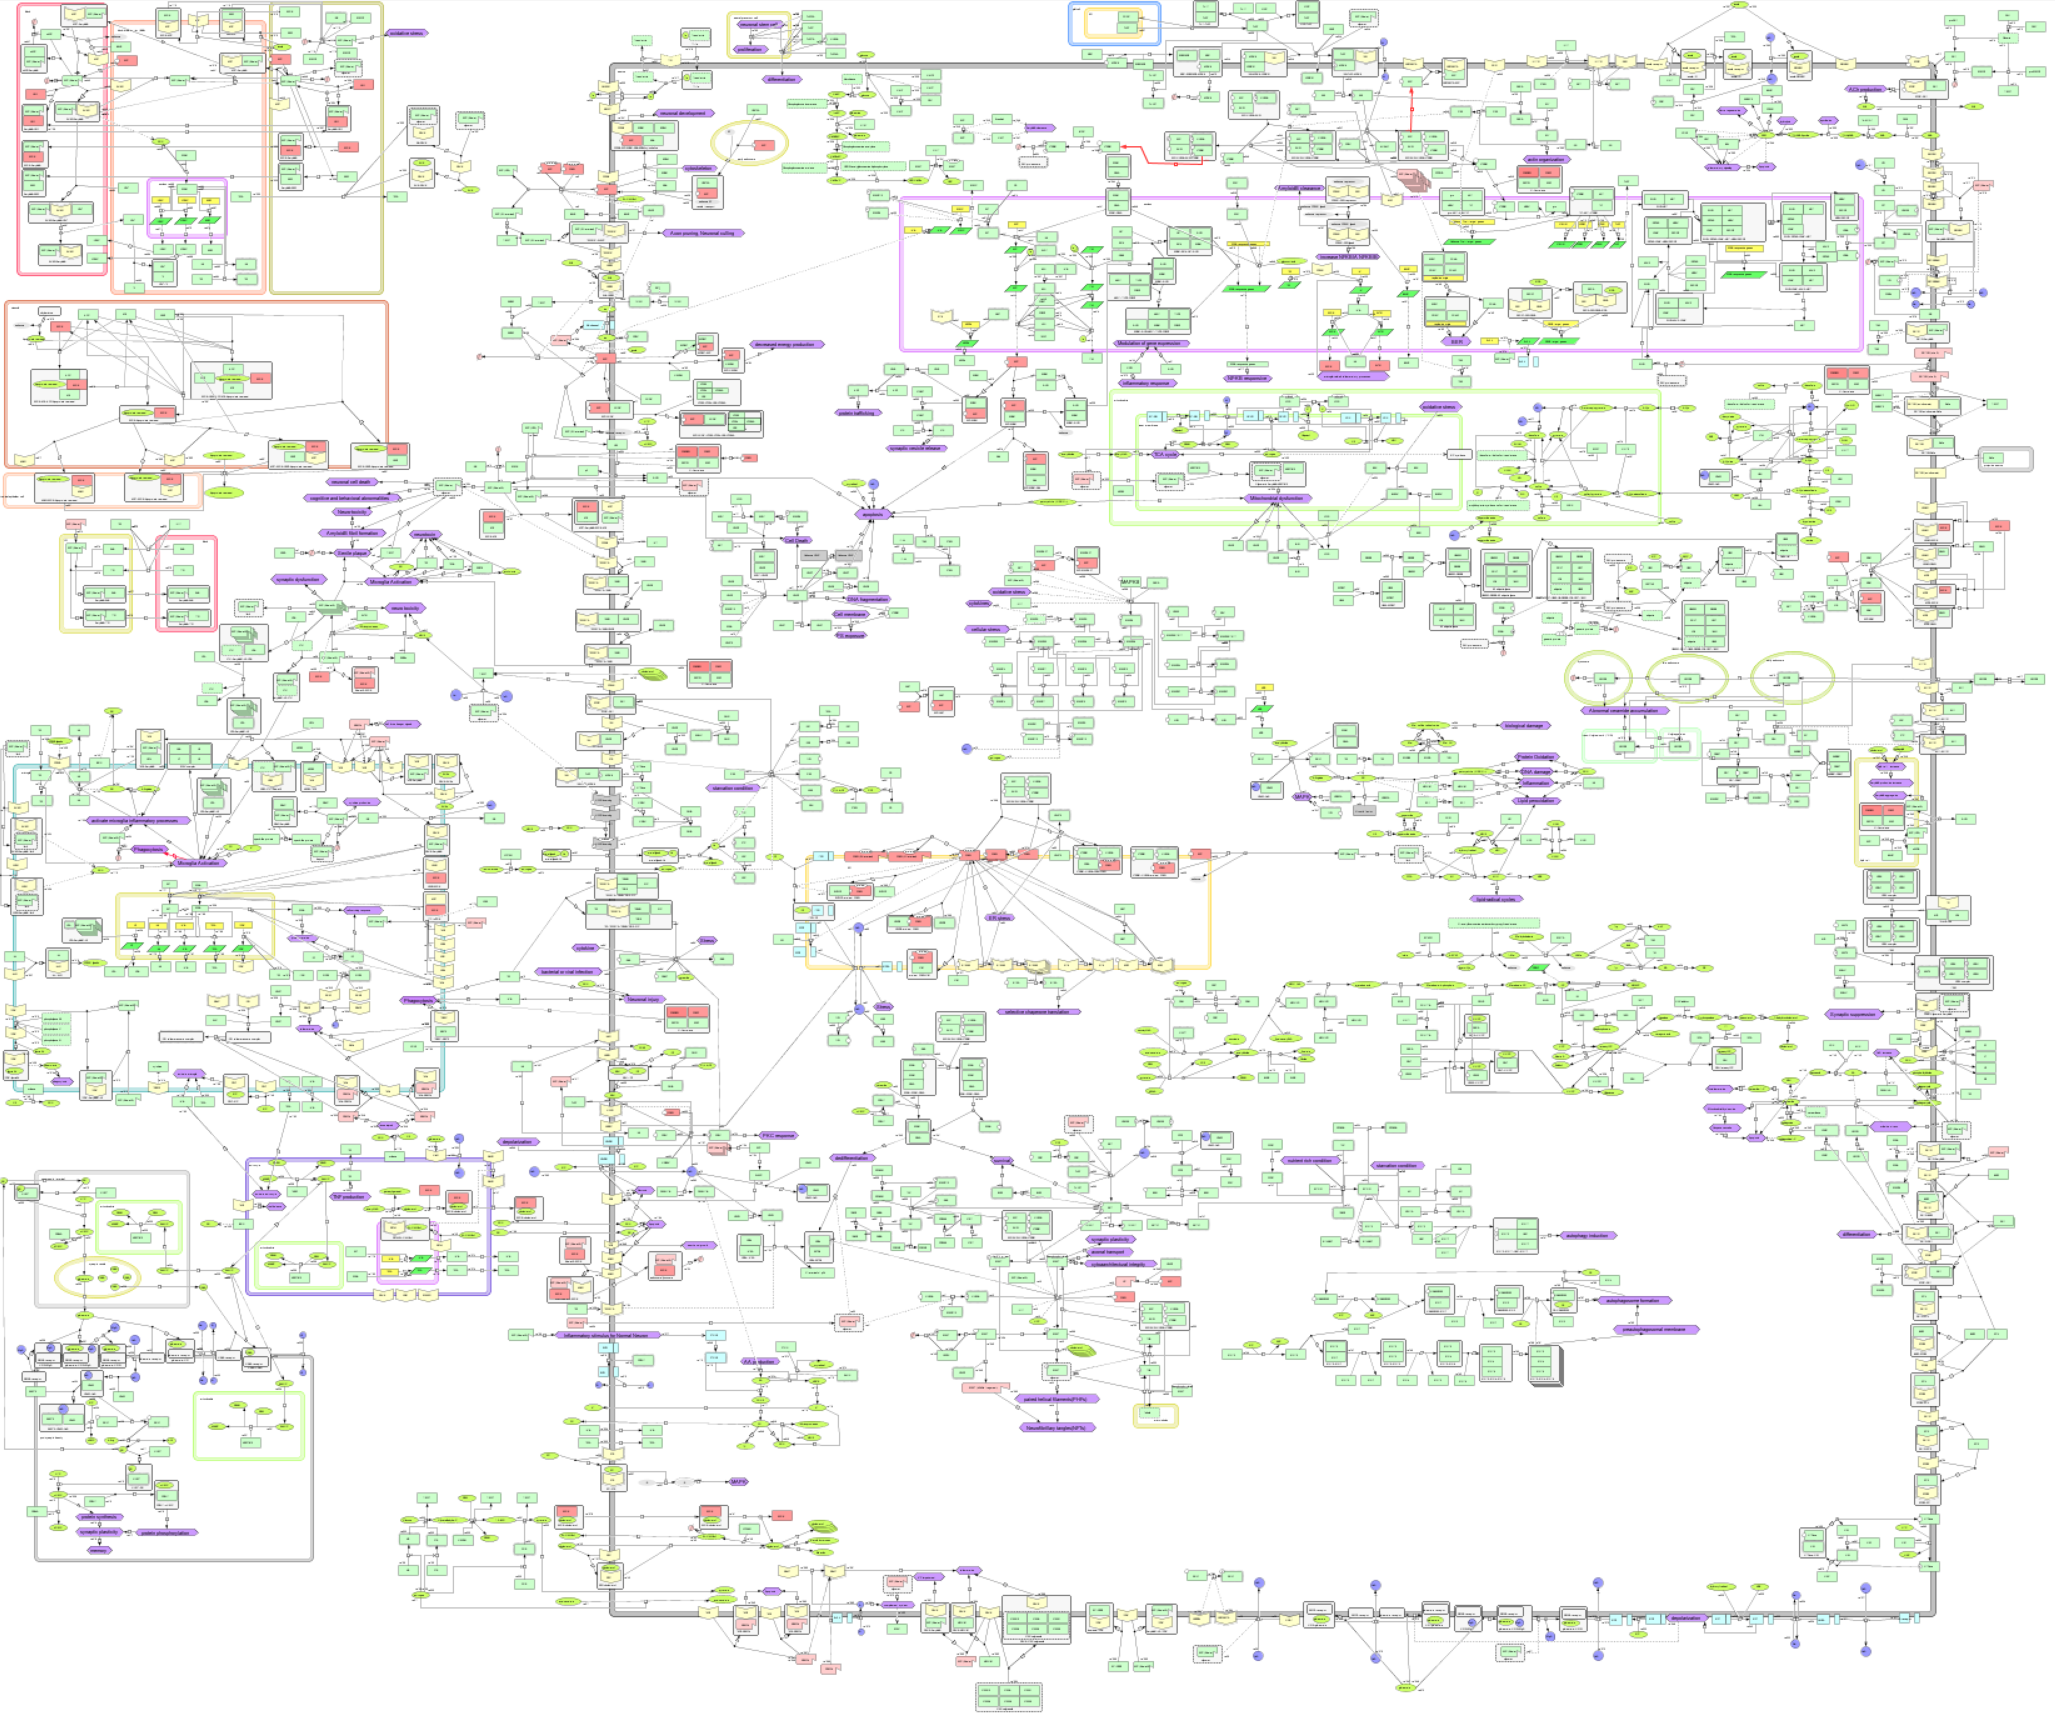
\includegraphics[height=0.9\textheight]{disease-map-screenshots/alzpathway-406.png}
    \caption{Zoomed-out view of the
      \textit{AlzPathway} disease map, a diagram describing biological processes
      related to Alzheimer's
      Disease~\cite{ostaszewski_AlzPathwayRegorganisationSteps_2021}.
    }%
    % \label{fig:disease-map-example}
  \end{figure}
  % TODO example of finished disease map, define species, species alias,
  % process/reaction/interaction, compartment, species types?
\end{frame}

\begin{frame}
  \frametitle{Introduction / Disease Maps}
  \begin{columns}
    \column{0.55\textwidth}
    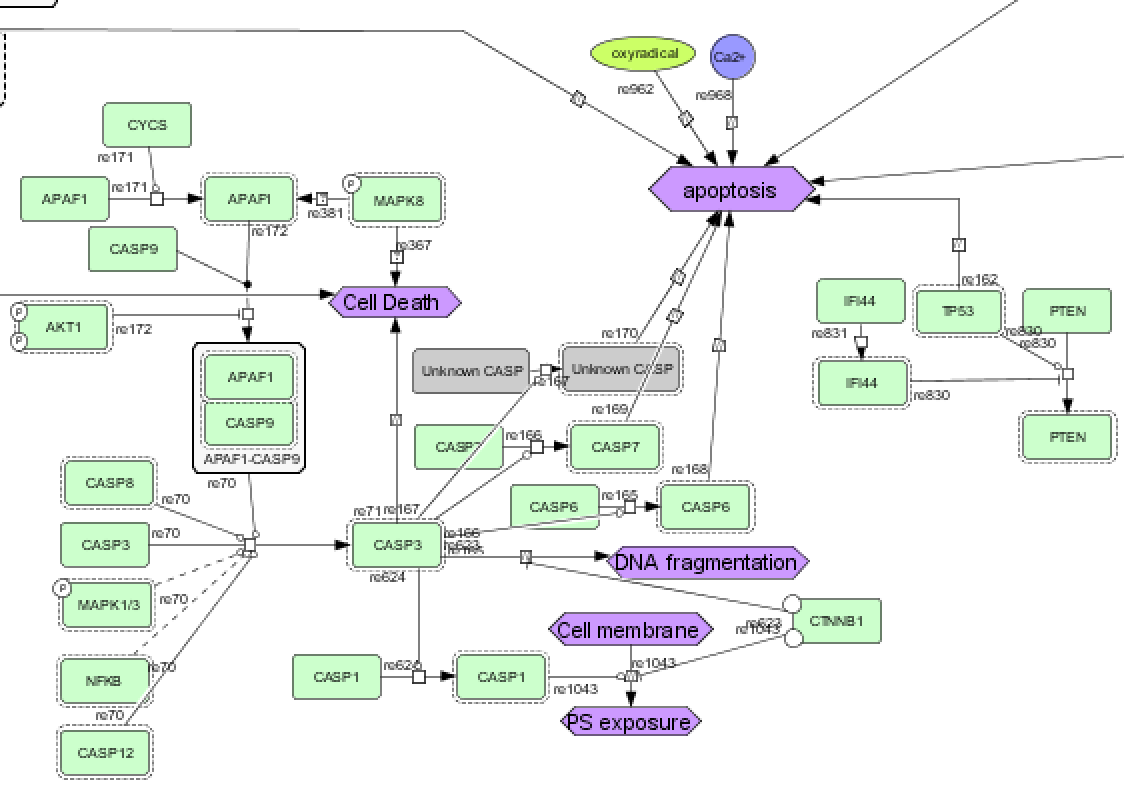
\includegraphics[width=\linewidth]{disease-map-screenshots/alzpathway-406-detail-1.png}
    \column{0.45\textwidth}
    \begin{definitionblock}{}
      \begin{itemize}
      \item \ild{species alias}: visual representation of biological actor (\ild{species})
      \item \ild{process}: interaction, relationship between species aliases
      \item complex species aliases: groups
      \item compartment boundaries
      \end{itemize}
    \end{definitionblock}

    \begin{observationblock}{}
      Can be interpreted as \textbf{attributed, bipartite graph} of species
      aliases and processes
    \end{observationblock}
  \end{columns}
\end{frame}

\begin{frame}
  \frametitle{Introduction / Disease Maps}
  \begin{columns}
    \column{0.55\textwidth}
    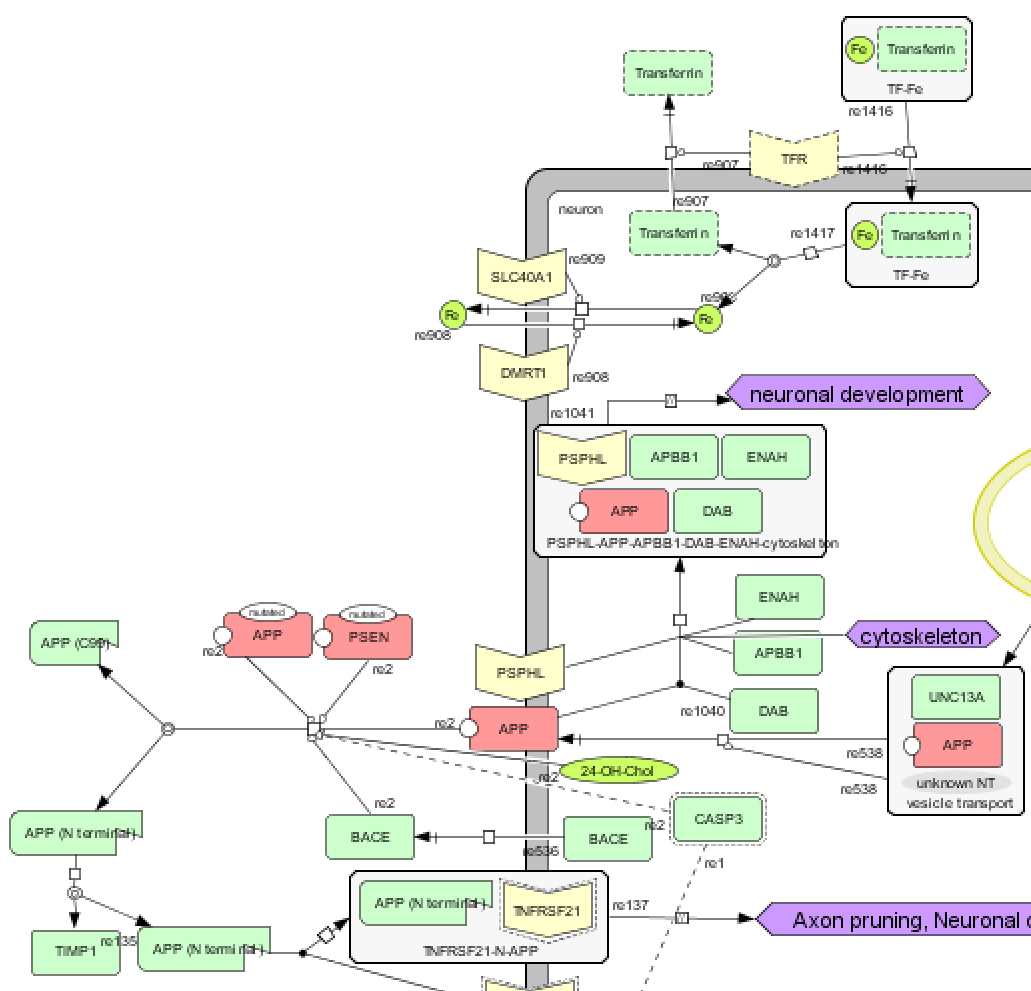
\includegraphics[width=\linewidth]{disease-map-screenshots/alzpathway-406-detail-2.png}
    % 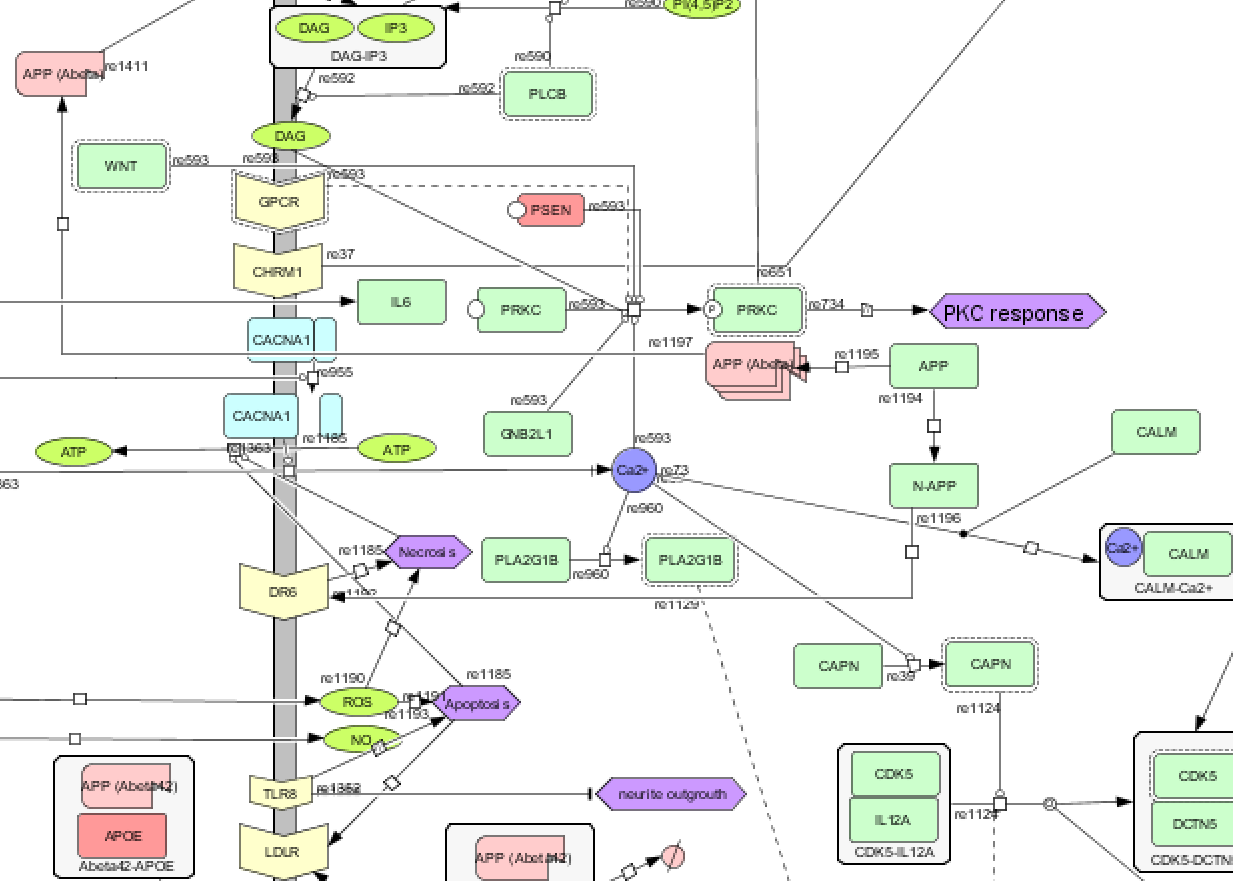
\includegraphics[width=\linewidth]{disease-map-screenshots/alzpathway-406-detail-4.png}
    \column{0.45\textwidth}
    \small
    Network structure and layout need to convey complex information faithfully:
    \begin{itemize}
      \small
    \item Different kinds of connections
    \item complexes, compartments
    \item visual hierarchy
    \item layout constraints for specific subgraphs (line, circle)
    \item represent species by multiple aliases
    \item ...
    \end{itemize}
    \begin{observationblock}{}
      Creating disease maps still involves considerable manual
      effort by domain expert
    \end{observationblock}
  \end{columns}
\end{frame}



\begin{frame}
  \frametitle{Introduction / Problem Statement}
  \begin{columns}
    \column{0.55\textwidth}
    % 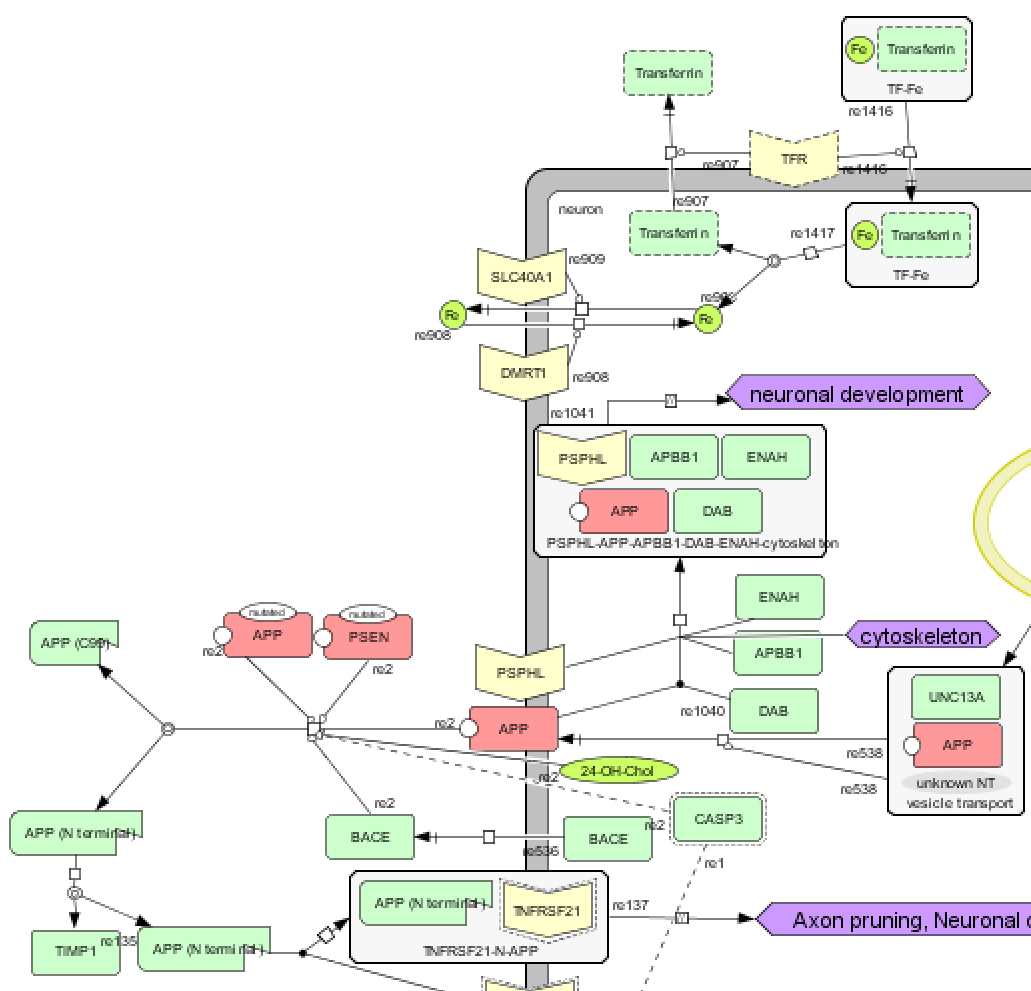
\includegraphics[width=\linewidth]{disease-map-screenshots/alzpathway-406-detail-2.png}
    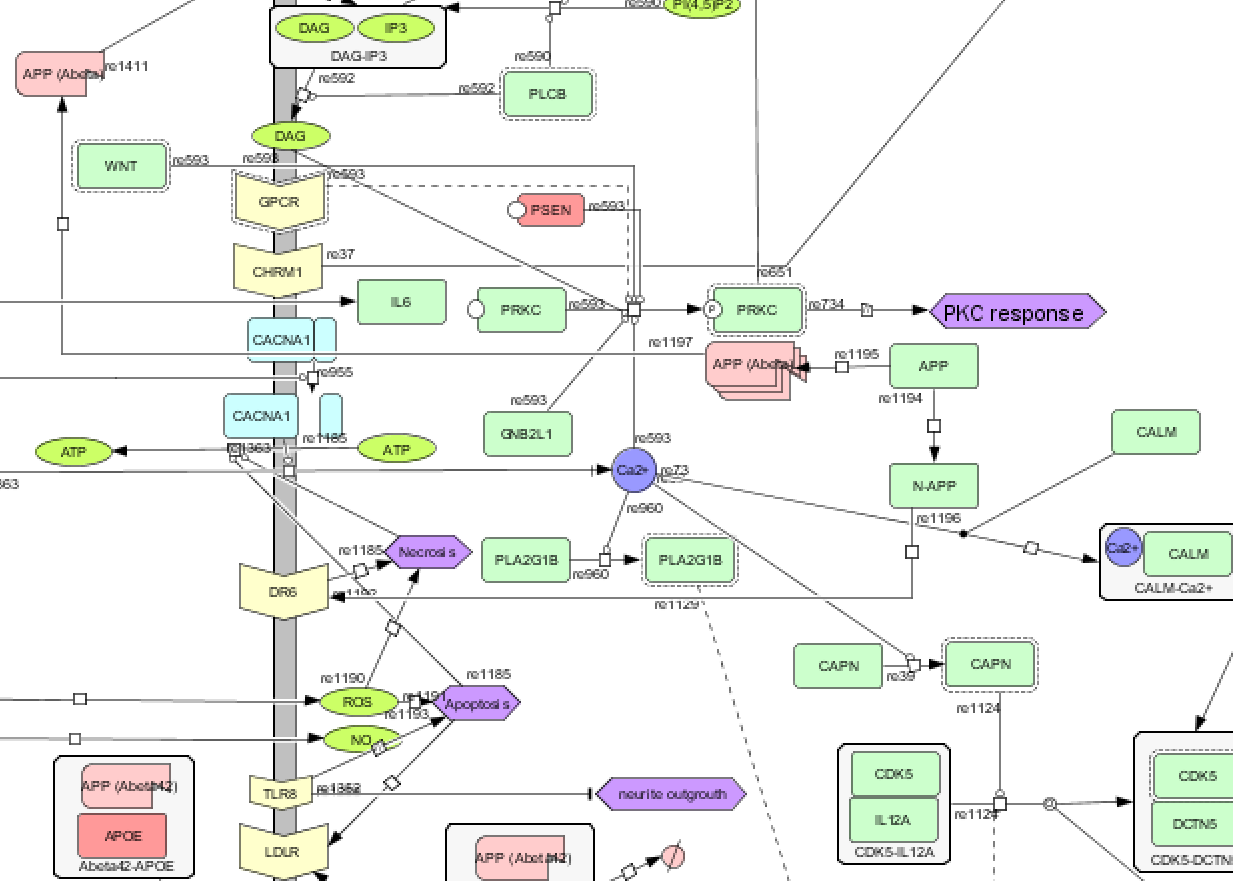
\includegraphics[width=\linewidth]{disease-map-screenshots/alzpathway-406-detail-4.png}
    \column{0.45\textwidth}
    \small
    \begin{itemize}
    \item A species alias may be connecting multiple processes
    \item This may be intentional
    \item ... or artifact of combining several subgraphs
    \end{itemize}
  \end{columns}
\end{frame}

% \begin{frame}
%   \frametitle{Introduction / Disease Maps / Examples}
%   \begin{columns}
%     \halfcol
%     \begin{figure}[h]
%       \centering
%       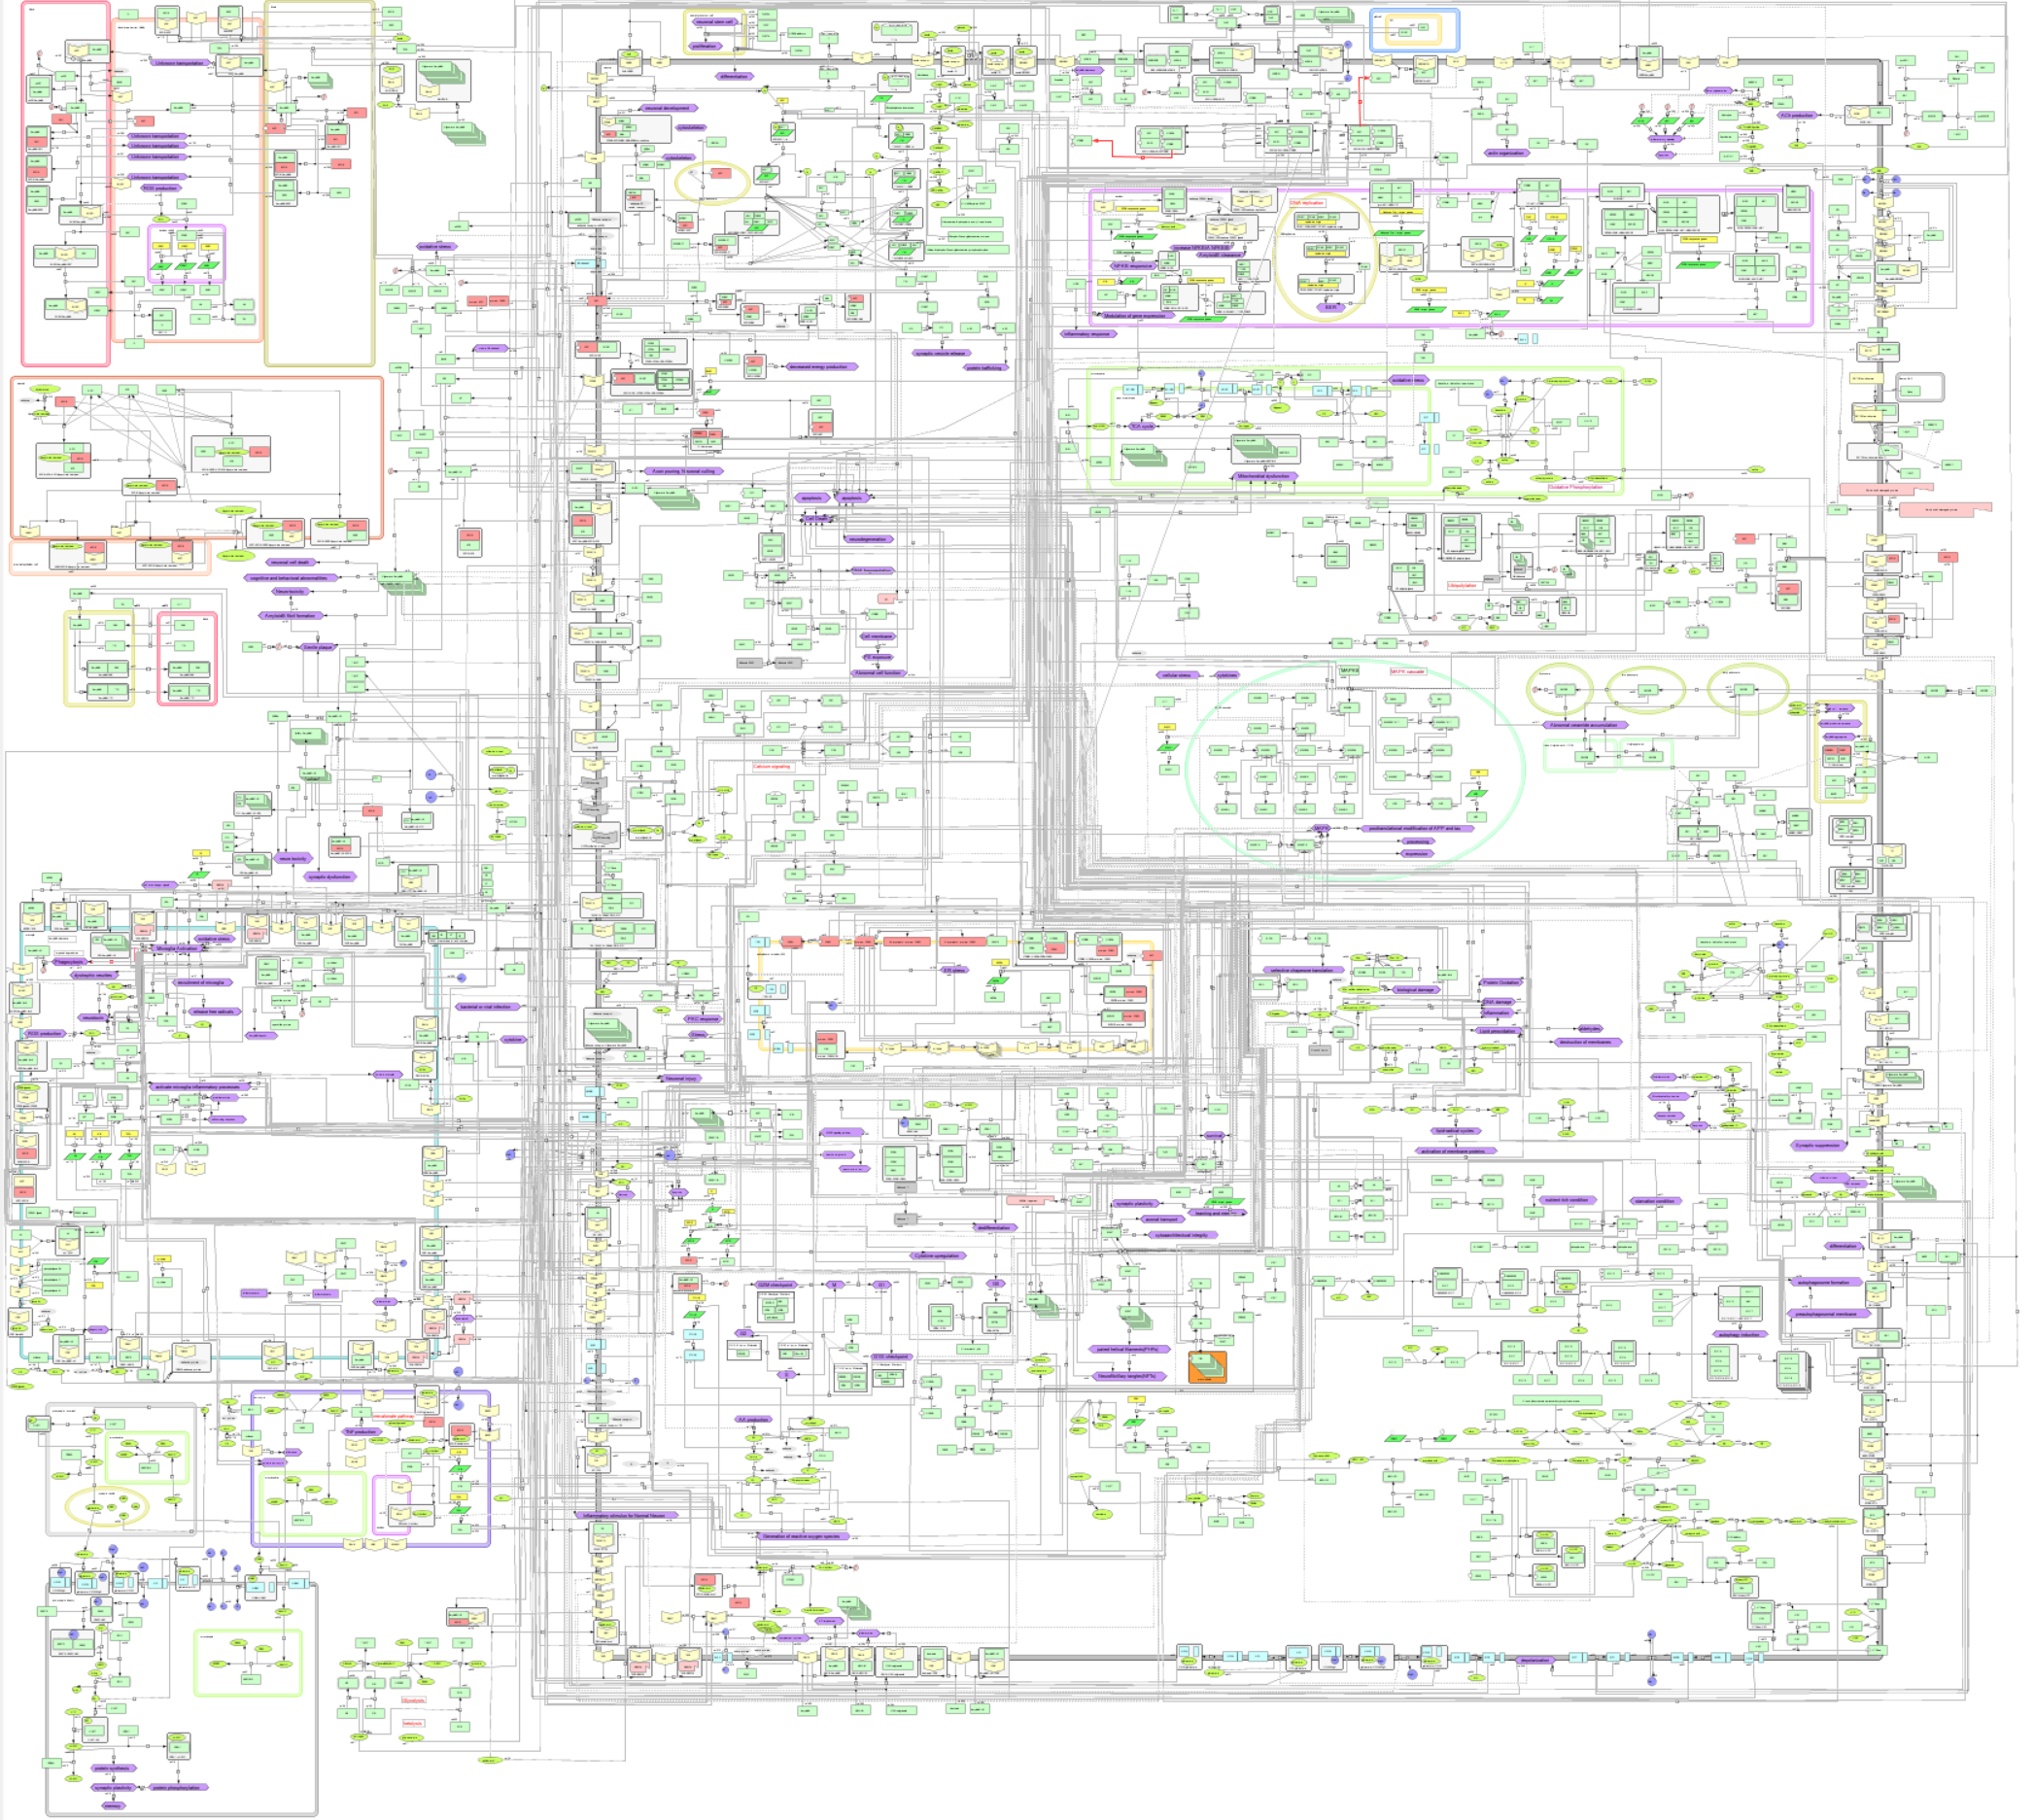
\includegraphics[width=\linewidth]{disease-map-screenshots/alzpathway/201.png}
%     \end{figure}
%     \halfcol
%     \begin{itemize}
%     \item Can always make layout task easier by duplicating nodes with degree
%       $\geq 2$
%     \item But which nodes can be duplicated s.t. network information remains faithful?
%     \end{itemize}
%   \end{columns}
% \end{frame}

\begin{frame}
  \frametitle{Introduction / Problem Statement}

  \begin{tabular}{C{2.8cm}  L{10cm}}
    % TODO add some words about how this is likely due to the interconnecte
    % nature of biological systems?
    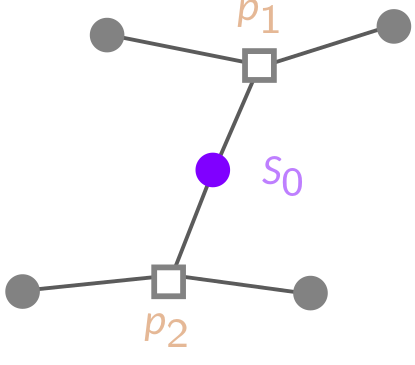
\includegraphics[width=0.7\linewidth]{true-false-connectivity-connected.png} &
                                                                                   To obtain an informative network structure, we need to distuingish... \\[3em]
                                                                                   % 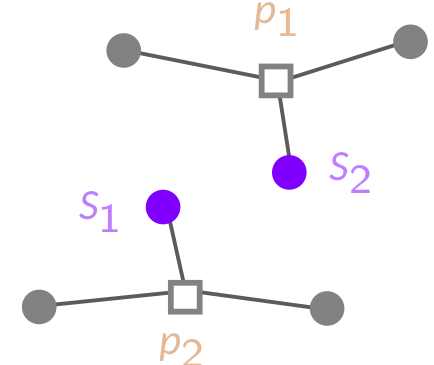
\includegraphics[width=0.7\linewidth]{true-false-connectivity-duplicated.png} & Path $(p_1, S_0, p_2)$ is not meaningful $\leadsto$ \ild{duplicate} $S_0$ \\[4em]
                                                                                   % 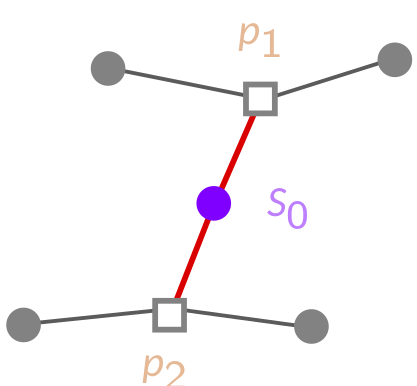
\includegraphics[width=0.7\linewidth]{true-false-connectivity-key-connector} & Path is meaningful $\leadsto$ $S_0$ must not be duplicated
  \end{tabular}

  \begin{definitionblock}{}
    \vspace{0.5em}
    \begin{columns}
      \column{8.5cm}
      Path $(p_1, S_0, p_2)$ is semantically meaningful
      (\ild{true connectivity})
      \\[1em]
      {
        % \footnotesize
        $\leadsto$ $S_0$ must not be duplicated
      }
      \column{2.8cm}
      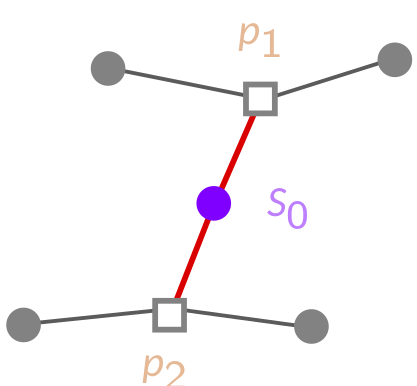
\includegraphics[width=0.7\linewidth]{true-false-connectivity-key-connector.png}
    \end{columns}
    \vspace{0.5em}
  \end{definitionblock}


  \begin{definitionblock}{}
    \vspace{0.5em}
    \begin{columns}
      \column{8.5cm}
      Path $(p_1, S_0, p_2)$ is not meaningful (\ild{false connectivity})
      \\[1em]
      {
        % \footnotesize
        There should be no paths implying false connectivity \\[0.5em] $\leadsto$ $S_0$ should be \ild{duplicated}
      }
      % TODO here we sort of pre-empt criteria for duplication
      \column{2.8cm}
      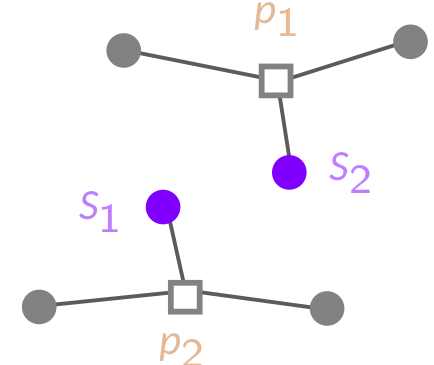
\includegraphics[width=0.7\linewidth]{true-false-connectivity-duplicated.png}
    \end{columns}
    \vspace{0.5em}
  \end{definitionblock}
  {\footnotesize
    e.g. due to unrelated roles of $S_0$ in $p_1$, $p_2$, not stoichiometrically
    linked, unimportant byproduct
  }

\end{frame}


\begin{frame}
  \frametitle{Introduction / Problem Statement}
  \small
  % Here, we consider...
  \begin{objectiveblock}{Objective 1}
    \vspace{0.5em}
    Assess whether a given species alias implies false connectivity (and should
    thus be duplicated)
    \vspace{0.5em}
  \end{objectiveblock}
  % TODO here: depends on context etc.?
  \vspace{1.5em}
  \begin{objectiveblock}{Objective 2}
    \vspace{0.5em}
    Determine number of duplicates and attachment of edges
    \vspace{0.5em}
  \end{objectiveblock}
  % TODO distinction between these two tasks...?
\end{frame}


\begin{frame}
  \frametitle{Related Work}

  \begin{objectiveblock}{Objective 1}
    Assess whether a given species alias implies false connectivity (and should
    thus be duplicated)
  \end{objectiveblock}
  
  Previous approaches would rely on \textbf{node centrality scores}

  \vspace{0.5em}

  \textcolor{gray}{
    \footnotesize
    high centrality $\leadsto$ heterogeneous neighbourhood $\leadsto$ false
    connectivity
  }

  \vspace{1.5em}

  \begin{itemize}
  \item node degree
    \cite{ma_ReconstructionMetabolicNetworks_2003, schuster_exploring_2002}
  \item eigenvector centrality
    \cite{manipur_clustering_2020}
  \item communities (modularity)
    \begin{itemize}
    \item contribution to modularity if node removed
      \cite{huss_CurrencyCommodityMetabolites_2007}
    \item based on intra- \& inter-community degrees
      \cite{guimera_FunctionalCartographyComplex_2005}
    \end{itemize}
  \item communities (semantic)
    \begin{itemize}
    \item cellular compartment
      \cite{manipur_clustering_2020}
    \item pathway annotation
      \cite{rohrschneider_NovelGridBasedVisualization_2010,joshi-tope_ReactomeKnowledgebaseBiological_2005,lambert_PathwayPreservingRepresentation_2011}
    \end{itemize}
  \end{itemize}
\end{frame}


\begin{frame}
  \frametitle{Problem Definition}
  % think: challenges in the problem and limitations of current approach
  % TODO still have to specify threshold
  % TODO still have to decide how many duplicates
  \begin{objectiveblock}{Objective 1}
    Assess whether a given species alias implies false connectivity (and should
    thus be duplicated)
  \end{objectiveblock}
  \begin{itemize}
  \item No clear requirements or guidelines (yet)
  \item Previous work relies on heuristic rules
  \end{itemize}
  % TODO factors that may make it hard to hand-craft rules
  \begin{itemize}
  \item Decision potentially depends on biological domain knowledge.
  \item[$\leadsto$] Try to learn rules from examples provided by domain expert \\
    \vspace{0.5em}
  \item Decision depends on \textit{context} (neighbourhood) of given species
    alias
  \item[$\leadsto$] Exploit information on graph structure
  \end{itemize}

  \vspace{1.5em}
  \begin{objectiveblock}{}
    Given \textbf{expert decisions}, train a ML model for \textbf{supervised node
      classification} to predict node duplication.
  \end{objectiveblock}
  % {\footnotesize
  % \begin{enumerate}
  % \item ``expert decisions''?
  % \item ``supervised node classification''?
  % \end{enumerate}
  % }
\end{frame}





\begin{frame}
  \frametitle{Data / Reorganisation Steps}
  \begin{itemize}
  \item \ild{AlzPathway} is a disease map that describes signalling
    pathways related to Alzheimer's Disease
  \item Recently received additional curation of layout, including duplication
    of nodes
  \item Snapshots of intermediate progress were saved (\ild{reorganisation
      steps}) \\
    {\footnotesize
      Total for 18 reorganisation steps, 6 of them involving node duplications
    }
  \end{itemize}
\end{frame}

\begin{frame}
  \frametitle{Data / Reorganisation Steps}
  \begin{figure}[h] \centering
    \includegraphics[height=0.95\textheight]{disease-map-screenshots/alzpathway/201-alzpath_18FEB.png}
  \end{figure}

\end{frame}


\begin{frame}
% %   \begin{figure}[h] \centering
%   %     \includegraphics[height=0.95\textheight]{disease-map-screenshots/alzpathway/202-alzpath_19FEB.png}
%   %   \end{figure}

%   %   \framebreak

  \begin{figure}[h] \centering
    \includegraphics[height=0.95\textheight]{disease-map-screenshots/alzpathway/406-alzpath_8APR.png}
  \end{figure}

\end{frame}



\begin{frame}
  % TODO move this after graph interpretation
  \frametitle{Data / Collapsed Maps}
    % dont really need this here, do we...
    % \begin{itemize}
    % \item
    %   Want to predict which nodes will be duplicated:
    %   \begin{itemize}
    %   \item Given sequence of graphs $(G_1, ..., G_k)$, infer ground-truth labels
    %     for nodes in $G_i$ by comparing to $G_{i+1}$
    %   \item Concatenation of $G_1, ..., G_{k-1}$ is input to classifier
    %     %     TODO this is just confusing...
    %   \end{itemize}
    % \end{itemize}
    \begin{itemize}
    \item Such reorganisation steps are hard to obtain in practice \\
      {\footnotesize Only given for \textit{AlzPathway}}
      \vspace{1.5em}
    \item For \textit{any} disease map graph, can create a single ``step'' by comparing it to its
      \ild{collapsed} version
      \begin{itemize}
      \item Replace all nodes (species aliases) corresponding to the same species with a single
        representative
      \item Attach all edges of aliases to representative
      \end{itemize}
      % TODO create picture for this
      \item Consider two additional maps
    \end{itemize}
\end{frame}





  % consider three disease maps...

  % \begin{frame}
  %   \frametitle{TODO}
  %   \begin{figure}[h]
  %     \centering
  %     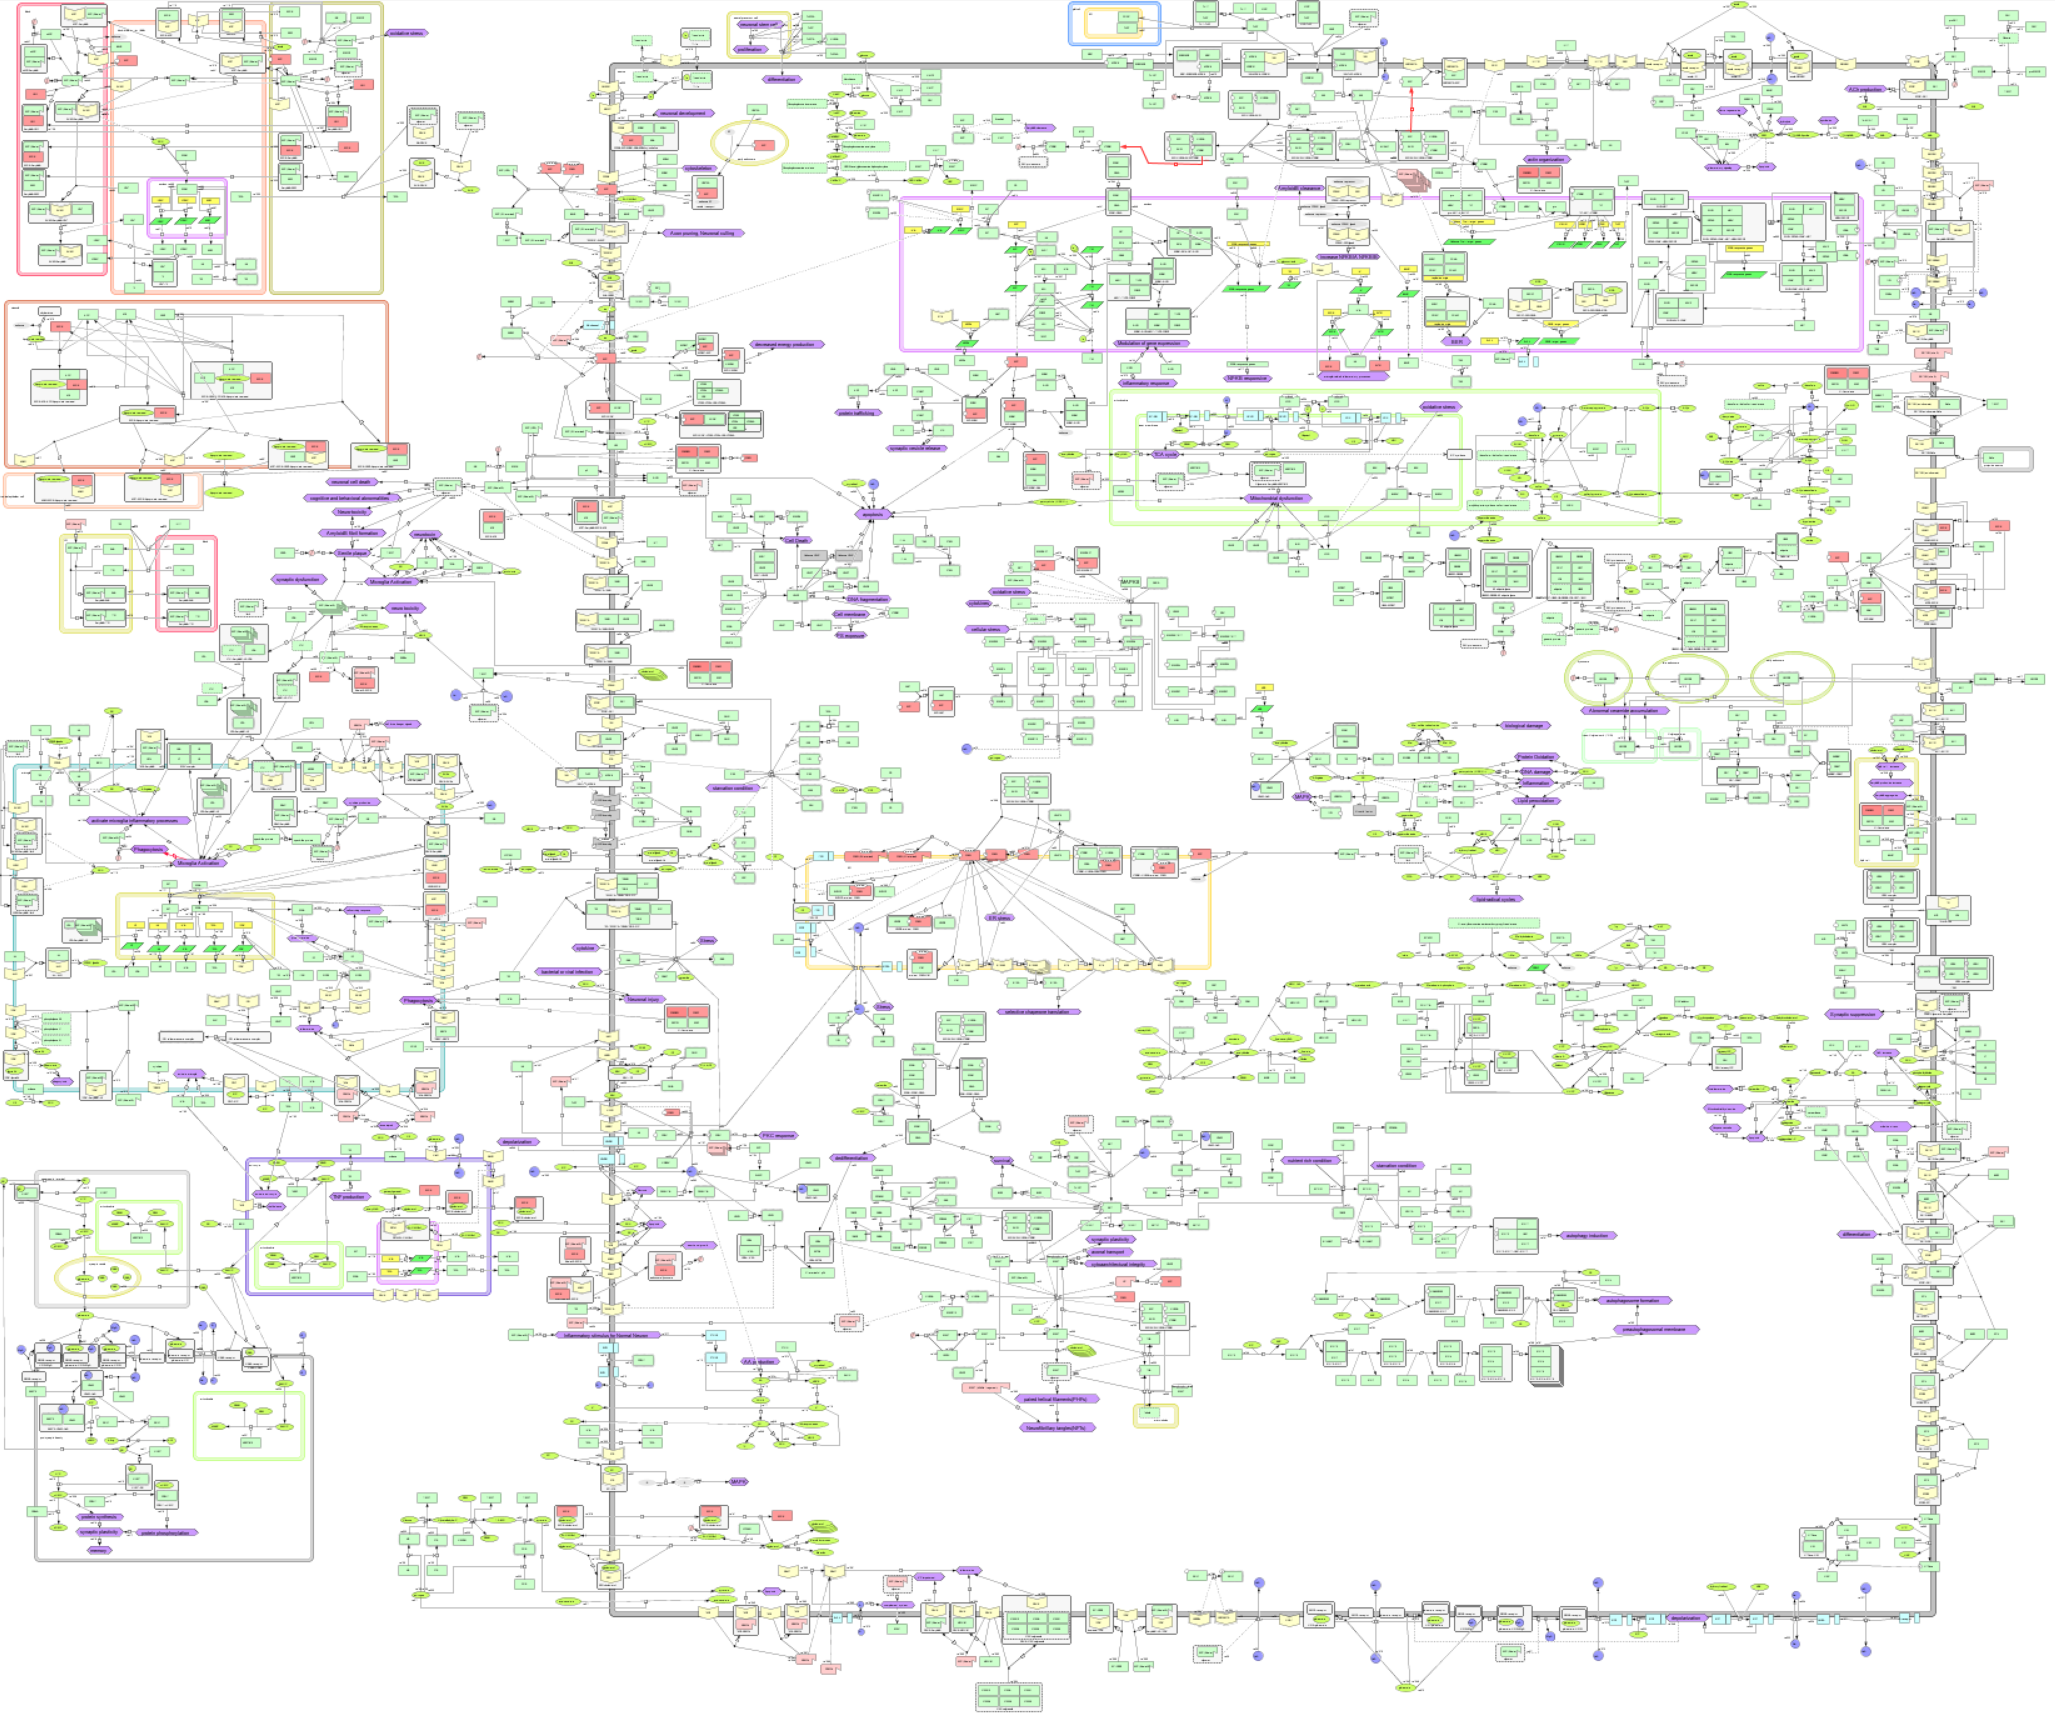
\includegraphics[width=0.6\linewidth]{disease-map-screenshots/alzpathway-406.png}
  %     \caption{ \textbf{AlzPathway}~\cite{mizuno_AlzPathwayComprehensiveMap_2012}
  %     describes signalling pathways related to Alzheimer's Disease
  %   }
  %   \end{figure}
  % \end{frame}

  \begin{frame}
    \frametitle{TODO}
    \begin{figure}[h]
      \centering
      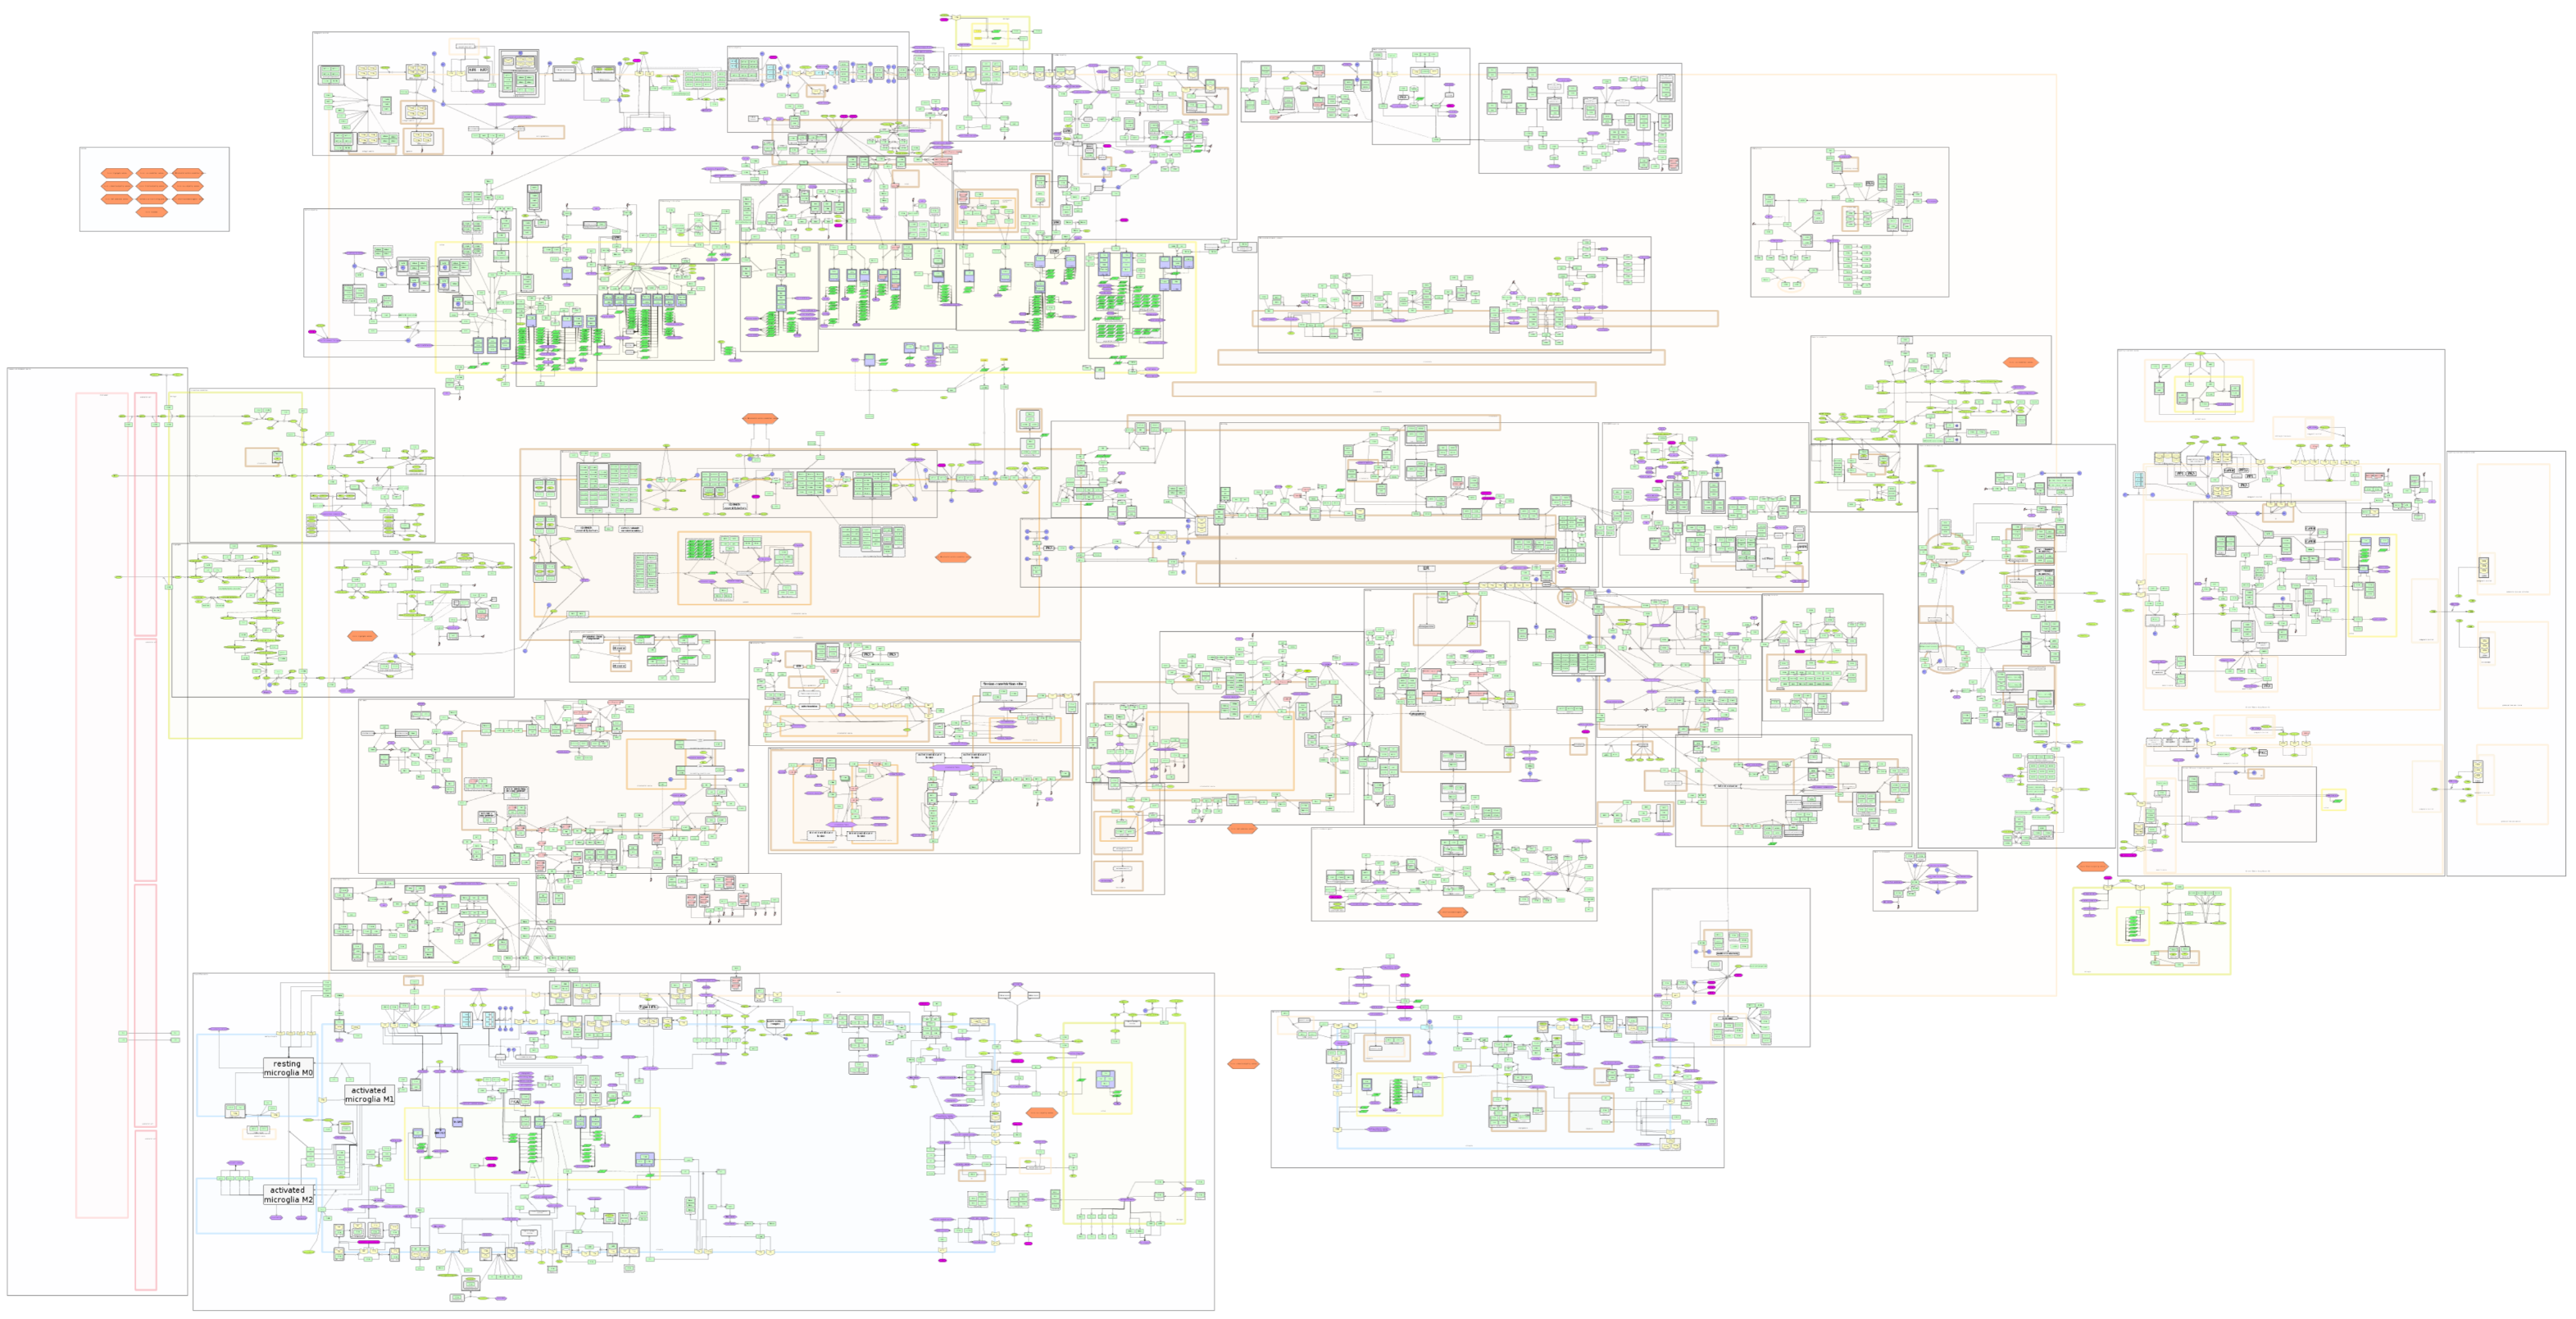
\includegraphics[width=\linewidth]{disease-map-screenshots/pdmap-whole}
      \caption{
        \textbf{Parkinson's Disease Map} (\PDMap{}) describes major pathways
        involved in pathogenesis of Parkinson's Disease
      }
    \end{figure}
  \end{frame}

  \begin{frame}
    \frametitle{TODO}
    \begin{figure}[h]
      \centering
      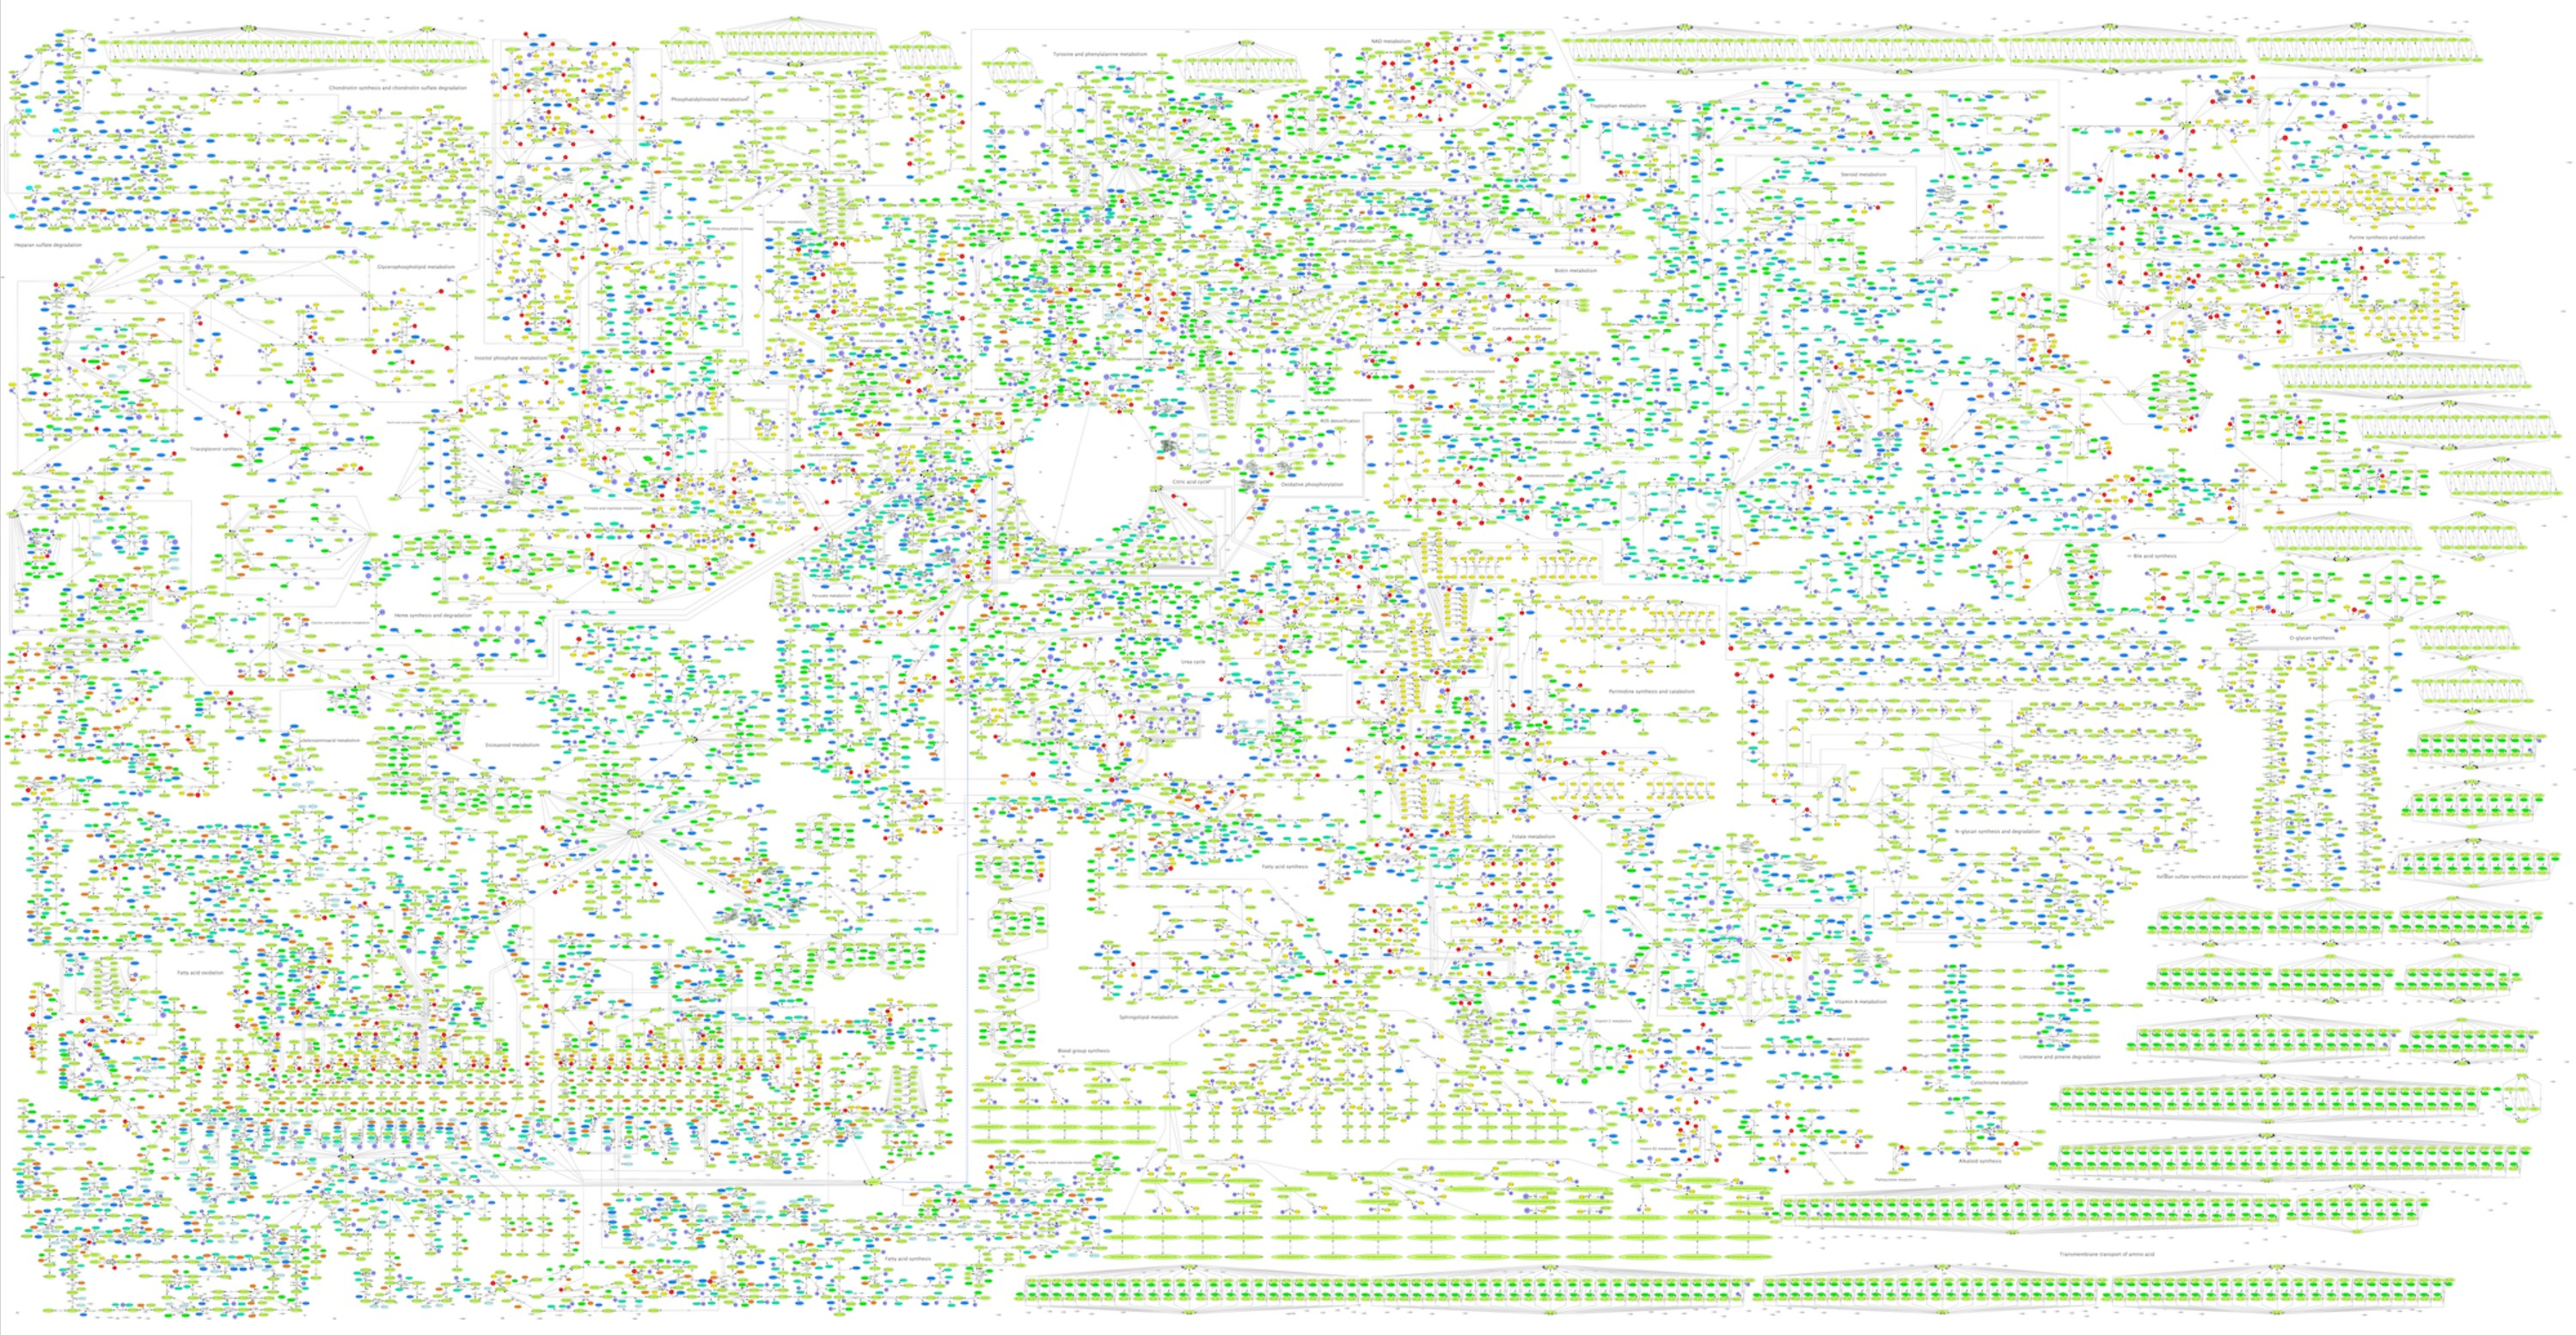
\includegraphics[width=\linewidth]{disease-map-screenshots/reconmap}
      \caption{
        \textbf{ReconMap}~\cite{noronha_ReconMapInteractiveVisualization_2017}, a
        visual representation of the \textit{Recon 2}~\cite{thiele_CommunitydrivenGlobalReconstruction_2013} GSMM }
    \end{figure}
  \end{frame}


  \begin{frame}
    \frametitle{TODO datasets used}

    \begin{figure}[h]
      \centering
      \begin{subfigure}{0.32\textwidth}
        % ADReorgLast summary
        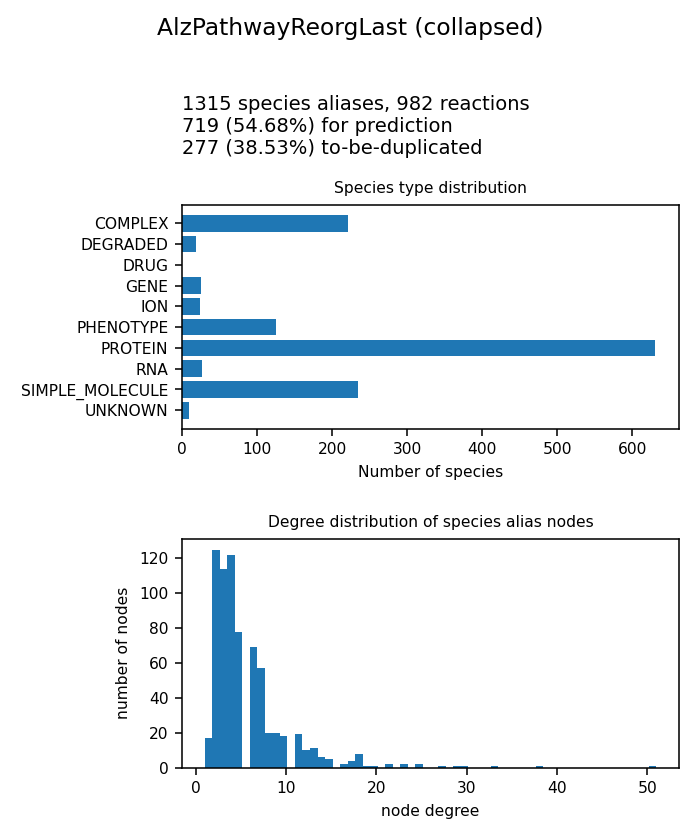
\includegraphics[width=\linewidth]{generated/AlzPathwayReorgLast.png}
      \end{subfigure}
      \begin{subfigure}{0.32\textwidth}
        % PDMap summary
        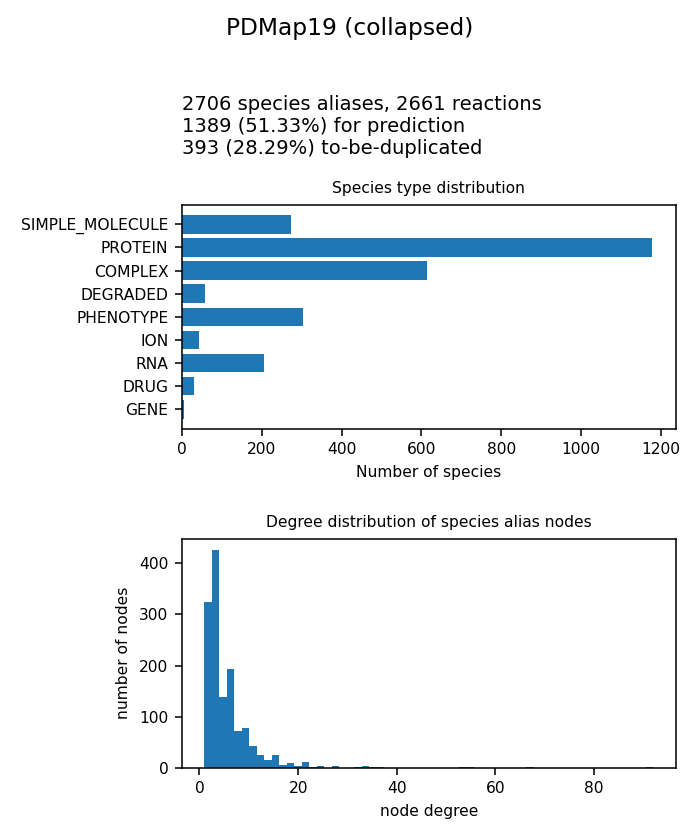
\includegraphics[width=\linewidth]{generated/PDMap19.png}
      \end{subfigure}
      \begin{subfigure}{0.32\textwidth}
        % ReconMap summary
        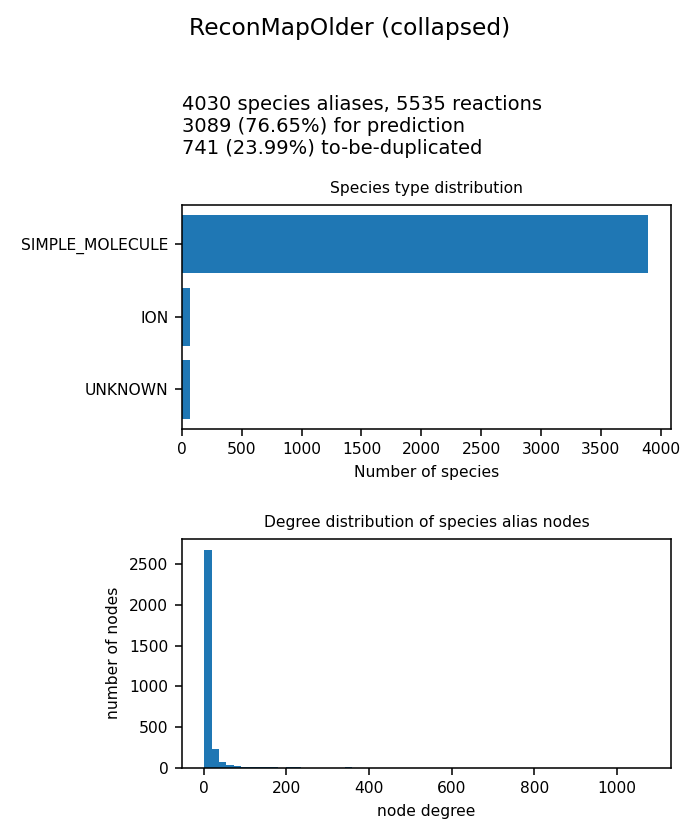
\includegraphics[width=\linewidth]{generated/ReconMapOlder.png}
      \end{subfigure}
      % \caption{An
      % overview of characteristics of the \textit{collapsed} networks used for
      % training: \ADLast{}, \PDMap{} and \ReconMap{}. The count of species aliases
      % and reactions is effectively the count of the bipartite node sets in the
      % constructed graphs.
      %   % Since we are considering collapsed diagrams, the count
      %   % of species aliases equals the count of species.
      % Networks and labels are
      % determined as described in \refsec{determining-labels}. Note that the $y$-axis of the
      % node degree histogram is plotted in logarithmic scale. \textit{ReconMap}
      % additionally has two nodes of degree $859$ and $1077$ that were excluded
      % from the histogram. }
      \label{fig:maps-summary}
    \end{figure}
  \end{frame}

  % TODO make notes about differences between DMs
  % TODO mention class imbalance
  % other challenges, here or later:
  % TODO contradictory, no always exhaustive
  % TODO reorganisations beyond node duplication


  \begin{frame}
    \begin{objectiveblock}{}
      Given \textbf{expert decisions}, train a ML model for \textbf{supervised node
        classification} to predict node duplication.
    \end{objectiveblock}

    % TODO somewhere 'round here introduce idea that we need to represent node by a
    % numerical feature vector and have different choices in constructing that.
    % (how do we even make this data available?) ``okay, so the plan is...''
    % maybe three diagrams: preprocessing, training and evaluation
    % TODO then probably here also note about how we dont do actual 'validation'
    % after model selection
    \vspace{1.5em}
    % TODO split this in preprocessing, training classifier and evaluating classifier
    % i.e. here, replace last part with indication that X, Y, A will be input to
    % some classifier
    \begin{figure}[h]
      \centering
      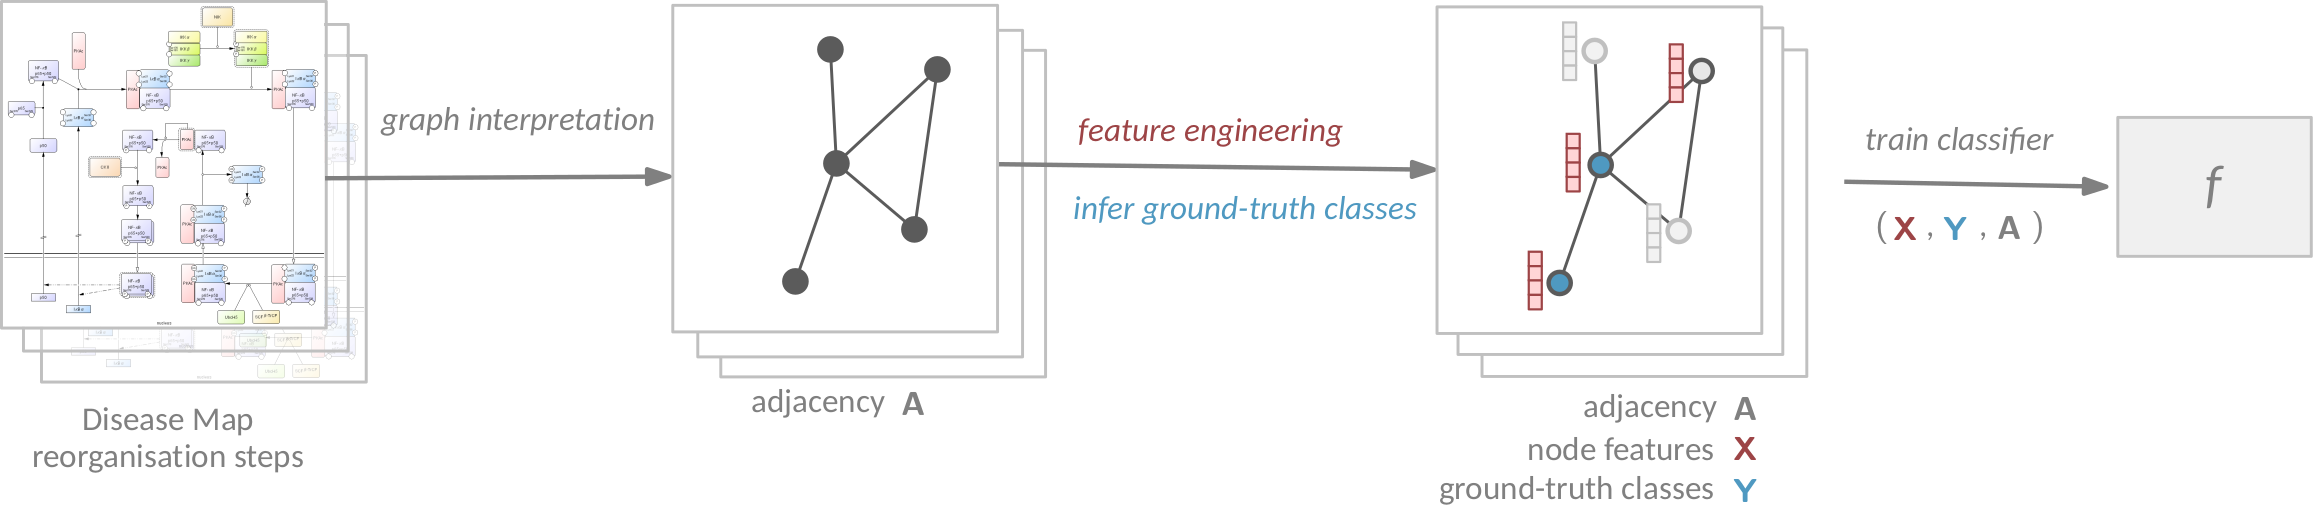
\includegraphics[width=0.95\textwidth]{pipeline-preprocessing.png}
    \end{figure}

  \end{frame}

  
  \begin{frame}
    \frametitle{Data / Graph Interpretation}
    \begin{enumerate}
    \item \textbf{Graph Interpretation}
      \begin{figure}[h] \centering
        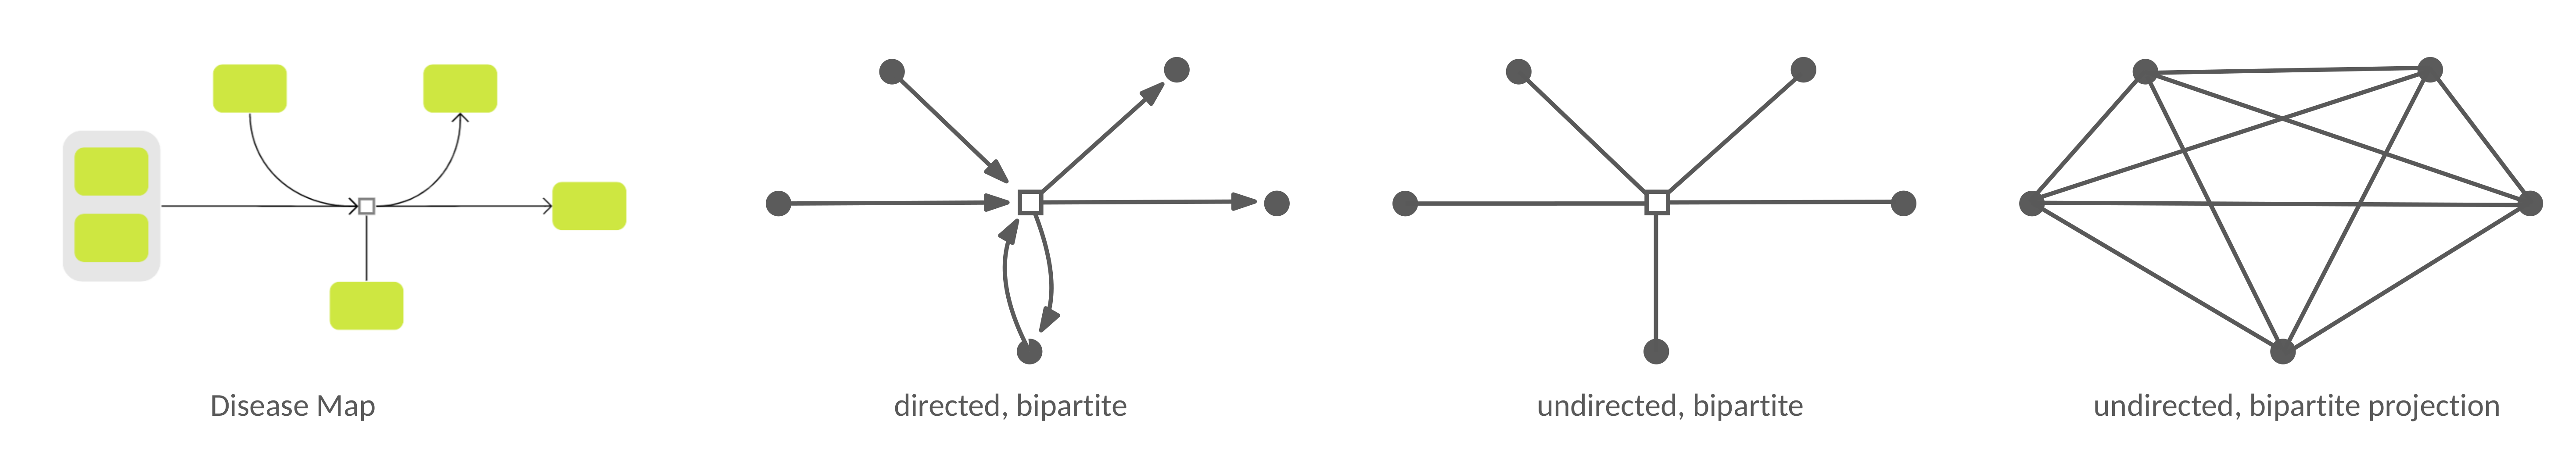
\includegraphics[width=\textwidth]{graph-interpretation-slides.png}
      \end{figure}
      \begin{itemize}
        \small
      \item Consider complex species aliases as single node
      \item No distinction between main substrates/products and side compounds
      \item Different interpretations for different situations
      \end{itemize}
      \vspace{1.5em}
    \item \textbf{Infer ground-truth labels}
      \begin{itemize}
        \small
      \item Compare to next step in reorganisation sequence to identify
        \textit{duplication parents}
      \end{itemize}
      \vspace{1.5em}
    \item[3. \& 4.] \textbf{Feature Engineering \& Classification}: in the following
      % \vspace{2em}
      % \item \textbf{Feature Engineering} 
      % \item \textbf{Training}
    \end{enumerate}
  \end{frame}

  
  \begin{frame}
    \frametitle{Problem Definition / Overview}
    \begin{objectiveblock}{}
      Given \textbf{expert decisions}, train a ML model for \textbf{supervised node
        classification} to predict node duplication.
    \end{objectiveblock}

    Recent work by
    \citeauthor{nielsen_MachineLearningSupport_2019}~\cite{nielsen_MachineLearningSupport_2019}:
    \begin{itemize}
    \item Node features based on graph centralities
      % \item Ground-truth labels based on reorganisation steps
    \item Consider collapsed map plus reorganisation steps
    \item Supplied to Support Vector Machine classifier
    \end{itemize}
    \vspace{1.5em}
    We extend this in several directions:
    \begin{itemize}
    \item Explore different classifier (Graph Neural Networks)
    \item Explore importance of reorganisation steps
    \item Explore choice of features
    \item Heuristic for determining number of duplicates and edge attachment
    \end{itemize}
  \end{frame}





  \begin{frame}
    % TODO schematic for TPR, TPR
    \frametitle{Problem Definition / Evaluation of Classifiers}
    \begin{itemize}
    \item To compare classifiers, we need an \textbf{unbiased performance measure}
    \end{itemize}
    \begin{itemize}
    \item Classifiers used herein yield a \ild{confidence score} in $[0,1]$ for a given example
    \item Obtain concrete classification by setting a \ild{decision threshold}, yields...
    \end{itemize}
    \begin{definitionblock}{}
      \begin{itemize}
      \item \ild{True Positive Rate} (\TPR{}): $\nicefrac{\text{\# true
            positives}}{\text{\# actually positive}}$
      \item \ild{False Positive Rate} (\FPR{}): $\nicefrac{\text{\# false
            positives}}{\text{\# actually negative}}$
      \end{itemize}
    \end{definitionblock}
    \begin{figure}[h]
      \centering
      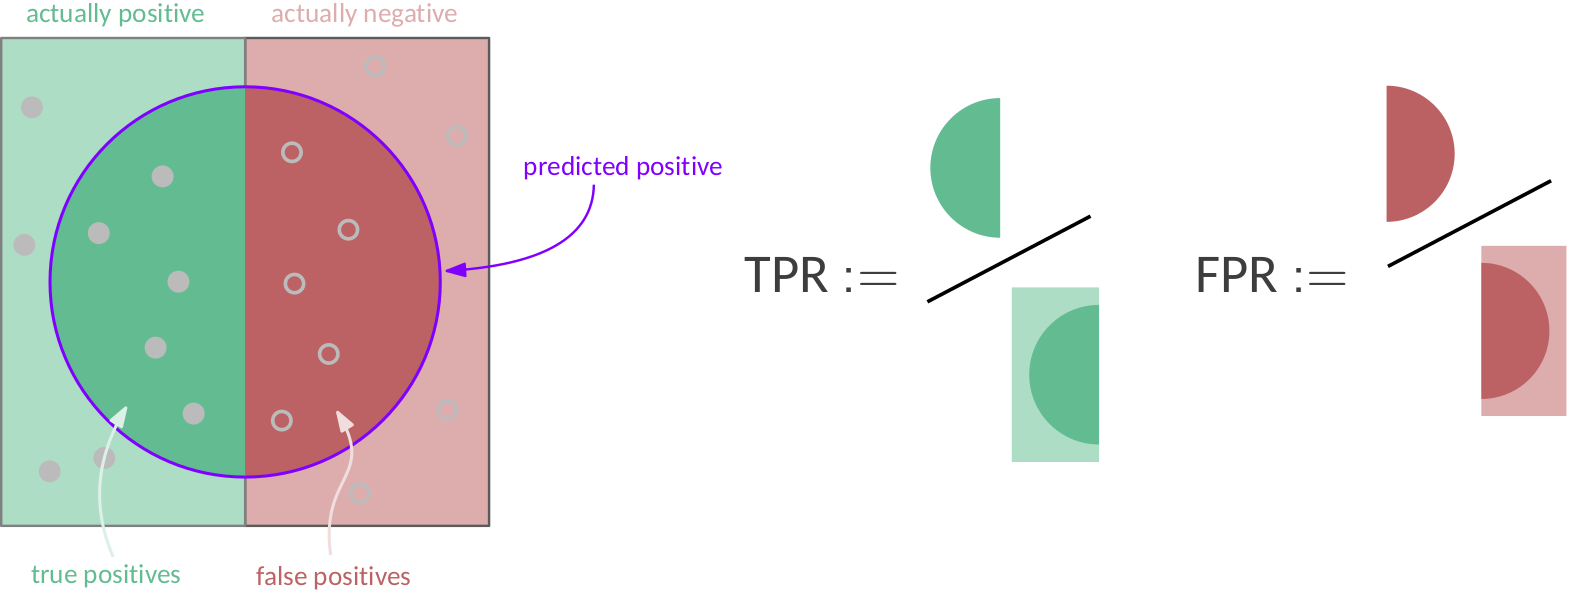
\includegraphics[width=0.7\textwidth]{tpr-fpr.png}
    \end{figure}
    % not analog. to precision-recall curve since recall is sensitive to
    % class skew  -- does not make sense to introduce Precision and Recall then,
    % simply stick to TPR, FPR


    \begin{itemize}
    \item Focus on positive class, Insensitive to class imbalance
    \end{itemize}
  \end{frame}

  % \begin{frame}
  %   \frametitle{Problem Definition / Evaluation of Classifiers / ROC Curve}
  %   \begin{columns}
  %     \halfcol
  %     \begin{figure}[h]
  %       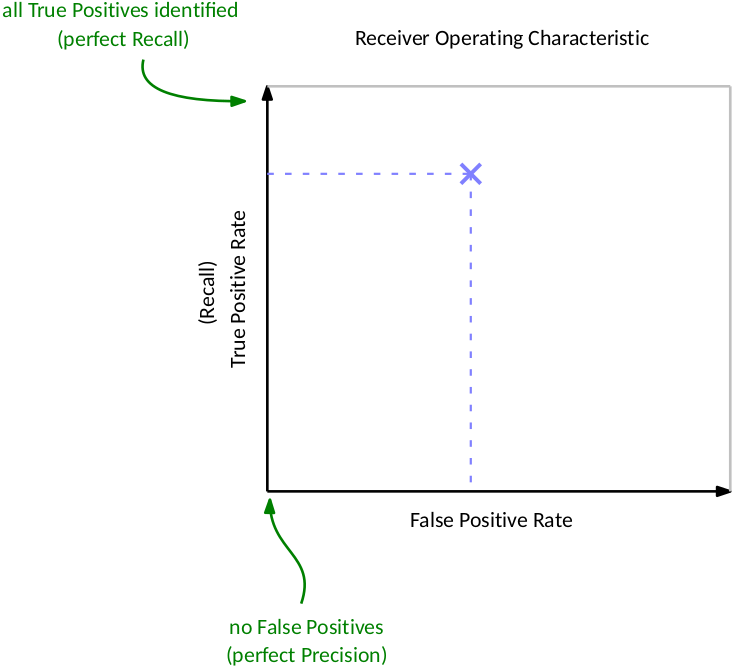
\includegraphics[width=7cm]{roc-intro.png}
  %     \end{figure}
  %     \halfcol
  %     \begin{itemize}
  %     \item Concrete choice of threshold yields binary classification and \TPR{}, \FPR{}
  %     \end{itemize}
  %   \end{columns}
  % \end{frame}

  \begin{frame}
    \frametitle{Problem Definition / Evaluation of Classifiers / ROC Curve}
    \begin{columns}
      \halfcol
      \begin{definitionblock}{}
        \ild{ROC Curve}: Plot \TPR{}, \FPR{} as function of decision threshold
      \end{definitionblock}
      \begin{itemize}
      \item Useful properties:
        \begin{itemize}
        \item Show overall behaviour with respect to variable threshold
        \item Insensitive to class distribution
          % If the proportion of positive to negative instances changes in a test set,
          % the ROC curves will not change.
        \item Insensitive to error costs
        \end{itemize}
      \item Usually a tradeoff, choice depends on use-case
        \begin{itemize}
          \footnotesize
        \item Accept only few high-confidence predictions $\rightarrow$ low
          \FPR{}, but also low \TPR{} (Recall)
        \item Lower decision threshold $\rightarrow$ increase \TPR{} at cost of
          increased \FPR{}
          % \item Accept only high-confidence predictions $\rightarrow$ high precision, low recall
          % \item Lower decision threshold $\rightarrow$ increase recall at cost of precision
        \end{itemize}
      \end{itemize}
      \halfcol
      \begin{figure}[h]
        % TODO move annotation in graphic s.t. less whitespace on left
        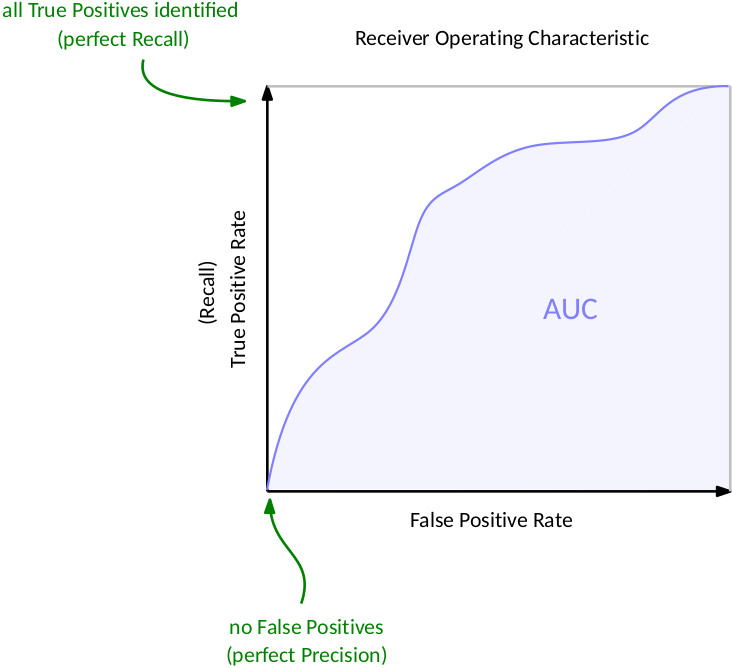
\includegraphics[width=7cm]{roc-intro-line.png}
        \caption{Plot \TPR{} and \FPR{} as function of decision threshold}
      \end{figure}
    \end{columns}
  \end{frame}

  \begin{frame}
    maybe recap slide here
    (then: ok, so now we have all the background we need to actually do stuff)
  \end{frame}







  \begin{frame}

    \frametitle{TODO Experiments / Reproducing / Features}

    Reproducing work of \citeauthor{nielsen_MachineLearningSupport_2019}:

    \vspace{1.5em}

    Features for a node $v$
    \begin{itemize}
    \item Centrality scores (degree, betweenness, closeness and eigenvector centrality)
    \item Statistics of centrality scores of neighbours (\textit{mean, min, max, stddev})
    \item Clustering coefficient
    \item One-hot encoding of species type
    \item Number of nodes $k$ hops from $v$ for $k \in \{1, ..., 5\}$,
      normalised by resp. count in grid graph.
    \end{itemize}

    \vspace{1.0em}

    \begin{itemize}
    \item Computed both on simple and bipartite graph interpretation where
      applicable
    \item Min-max normalised to $[0,1]$
    \end{itemize}

    \vspace{1.0em}

    \begin{itemize}
    \item \textbf{Train} on \textit{AlzPathway} reorganisation steps plus
      collapsed version of first step
    \item \textbf{Evaluate}  on \textit{PDMap} and \textit{ReconMap} (separately)
    \end{itemize}
  \end{frame}


  \begin{frame}
    % how much detail do we need here?
    % TODO dont show stuff about loss? if not, make that a bonus slide

    \frametitle{TODO Experiments / Reproducing / SVM / Results}
    % reproducing: show AUC comparison for PDMap, ROC curves for ReconMap
    \begin{figure}[h]
      \centering
      \begin{subfigure}[h]{0.49\linewidth}
        \centering
        \includegraphics[width=0.9\linewidth]{svm-repro-repeats/results/comparison/roc-svm-only.png}\\
        % TODO not include this table? 'theirs' number is super fishy and I would
        % invalidate it while speaking anyways
        \begin{tabular}[h]{l | l}
          & AUC \\ \hline
          SVM (theirs) & 0.69 \\
          SVM (ours) & 0.78
        \end{tabular}
        \caption{(\ADMap{} $\rightarrow$ \PDMap)}
      \end{subfigure}
      \begin{subfigure}[h]{0.49\linewidth}
        \centering
        \includegraphics[width=0.9\linewidth]{svm-repro-reconmapolder-repeats/results/comparison/roc-svm-only.png}\\
        \begin{tabular}[h]{l | l}
          & AUC \\ \hline
          SVM (theirs) & 0.76 \\
          SVM (ours) & 0.72
        \end{tabular}
        \caption{(\ADMap{} $\rightarrow$ \ReconMap)}
      \end{subfigure}
    \end{figure}
  \end{frame}
  % TODO here: general interpretation of ROC shape, i.e. 0.25 of all positives
  % with amost no false positives

  \begin{frame}

    \frametitle{TODO Experiments / Reproducing / SVM / Discussion}

    \begin{observationblock}{}
      \begin{itemize}
        % TODO somewhere make clear that we re-implement from scratch
      \item Our SVM implementation performs worse than that of
        \citeauthor{nielsen_MachineLearningSupport_2019}
        % TODO would be nice to have a definition block here for this
      \item Challenge when working with reorganisation steps:
        \textbf{contradictory examples}
      \end{itemize}
    \end{observationblock}
    \begin{itemize}
    \item Duplicated node has positive label in $G_k$ but negative label in
      $G_j$ for $j < k$
    \item Reasonable only if we can assume that in reorg. step, all critical
      nodes are in fact being duplicated
    \item Likely not the case in \textit{AlzPathway}, rather: simply not
      considered yet
      % TODO rethink logic
    \item If reorganisations have little impact on features of other nodes:
    \item[$\leadsto$] Two training examples with potentially similar features but different label
    \end{itemize}
    \begin{itemize}
    \item \citeauthor{nielsen_MachineLearningSupport_2019}: exclude negative examples that
      are within 1\% of feature space extent to ex. of positive class
    \item Here: Exclude node corresponding to positive example from previous
      reorganisation steps.
    \item More on this later
    \end{itemize}
  \end{frame}


  \begin{frame}

    \frametitle{Reproducing / GNN / Recap 1}

    \begin{columns}
      \column{0.7\textwidth}
      \begin{itemize}
      \item Basic idea: duplication depends not only on characteristics of single
        node but also on its \textit{context}
      \item GNN learns hidden representation of node based on its context.
      \end{itemize}
      \begin{definitionblock}{GNN blueprint}
        {\small
          New hidden representation of $v$ is result of
          convolution localised around $v$:
        }
        \begin{align*}
          & \vec h_i' \gets \textsc{Update}(\textsc{Agg}(\{\textsc{Msg}(\vec h_j, \vec h_i) ~|~ j \in \mathcal{N}_i\}))
        \end{align*}
        \begin{enumerate}
        \item \textsc{Msg}$(\vec h_j, \vec h_i)$: produce message from $v_j$ to $v_i$
        \item \textsc{Agg}$(...)$: combine messages received by neighbours
        \item \textsc{Update}$(...)$: combine aggregated messages with own state
        \end{enumerate}
      \end{definitionblock}

      % {\small
      % Simple GNN architectures:
      % \begin{itemize}
      % \item $\mathcal{N}_i$: 1-hop neighbourhood
      % \item $\textsc{Msg}(\vec h_j, \vec h_i) = \mathbf{W} \vec h_j$
      % \item $\textsc{Agg}(...) = \bigoplus_{j \in \mathcal{N}_i} \alpha_{ij}
      %   \textsc{Msg}(\vec h_j, \vec h_i)$
      %   \begin{itemize}
      %   \item[] $\bigoplus$: permutation-invariant agg., e.g. \textit{sum,
      %     mean, max}
      %   \end{itemize}
      % \item $\textsc{Update}(...)$: activation function $\sigma$
      % \end{itemize}

      % }
      \column{0.29\textwidth}
      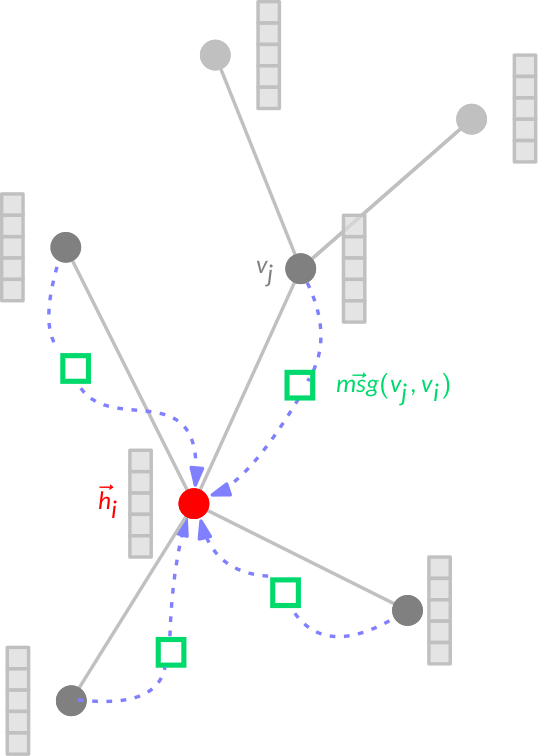
\includegraphics[width=\linewidth]{messagepassing.png}
    \end{columns}
  \end{frame}



  \begin{frame}

    \frametitle{Reproducing / GNN / Recap 2}

    \begin{columns}
      \column{0.7\textwidth}
      {\small
        Simple GNN architectures:
        \begin{itemize}
        \item $\mathcal{N}_i$: 1-hop neighbourhood
        \item $\textsc{Msg}(\vec h_j, \vec h_i) = \mathbf{W} \vec h_j$
        \item $\textsc{Agg}(...) = \bigoplus_{j \in \mathcal{N}_i} \alpha_{ij}
          \textsc{Msg}(\vec h_j, \vec h_i)$
          \begin{itemize}
          \item[] $\bigoplus$: permutation-invariant agg., e.g. \textit{sum,
              mean, max}
          \end{itemize}
        \item $\textsc{Update}(...)$: activation function $\sigma$
        \end{itemize}
      }
      \begin{definitionblock}{GNN models}
        \begin{itemize}
        \item \ild{GCN} \cite{kipf_graph_nodate}: $\alpha_{ij} =
          \nicefrac{1}{\sqrt{d_i d_j}}$
        \item \ild{GAT} \cite{velickovic_graph_2018}: $\alpha_{ij}$ determined
          by single-layer NN
          \begin{align*}
            e_{ij} & := \sigma_{\text{att}}(\vec a^T( \msg_i \concat \msg_j)) \\
            \alpha_{ij} &:= \softmax_{j \in \mathcal{N}_i}(e_{ij}) := \frac{\exp(e_{ij})}{\sum_{k \in \mathcal{N}_i} \exp(e_{ik})}
          \end{align*}

        \end{itemize}
      \end{definitionblock}
      \column{0.29\textwidth}
      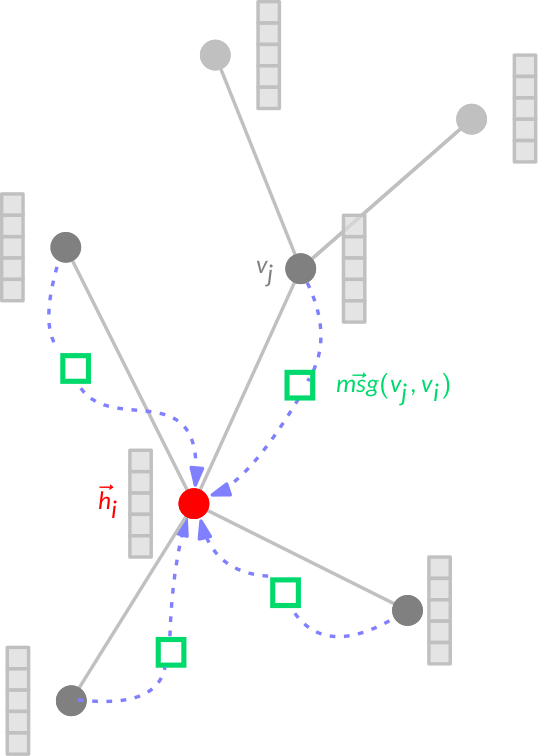
\includegraphics[width=\linewidth]{messagepassing.png}
    \end{columns}
  \end{frame}

  \begin{frame}
    \frametitle{Reproducing / GNN / Setup}
    {
      Apply GNN to previous task
      \begin{itemize}
      \item same input features
      \item message-passing on bipartite projection
      \end{itemize}
      Architecture:
      \begin{itemize}
      \item 2 message-passing layers
      \item 2 fully-connected layers before and after message-passing
      \end{itemize}
    }
    % TODO schematic of GNN model? but then we'd have to add skip connections...
  \end{frame}

  \begin{frame}
    \frametitle{Reproducing / GNN / Results}
    \begin{observationblock}{}
      \begin{itemize}
      \item \textit{PDMap}: GNN model is slightly better
      \item \textit{ReconMap}: outperforms our and their SVM
      \item Variablity w.r.t. random initialisation
      \end{itemize}
    \end{observationblock}
    \begin{figure}[h]
      \centering
      \begin{subfigure}[h]{0.49\linewidth}
        \centering
        \includegraphics[width=0.9\linewidth]{svm-repro-repeats/results/comparison/roc.png}
        \caption{(\ADMap{} $\rightarrow$ \PDMap)}
      \end{subfigure}
      \begin{subfigure}[h]{0.49\linewidth}
        \centering
        \includegraphics[width=0.9\linewidth]{svm-repro-reconmapolder-repeats/results/comparison/roc.png}
        \caption{(\ADMap{} $\rightarrow$ \ReconMap)}
      \end{subfigure}
    \end{figure}
  \end{frame}

  \begin{frame}
    \frametitle{Experiments / Importance of Reorganisation Steps / Introduction}
    \begin{itemize}
    \item Note that we are evaluating on single collapsed disease maps
    \item ... but are also using reorganisation steps for training
    \end{itemize}
    % however, if you look at this graph....
    \begin{figure}[h]
      \centering
      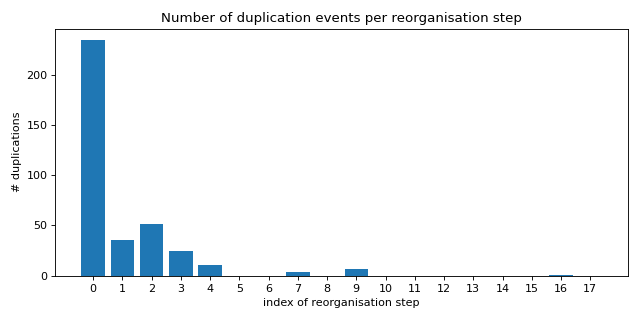
\includegraphics[width=0.4\textwidth]{dupcounts.png}
    \end{figure}
    \begin{itemize}
    \item most duplication events due to step from collapsed map
    \item node features in later reorganisation steps may be different from
      typical features of collapsed maps
    \item amplifies class imbalance
    \item need to consider evaluation methods and use-case
    \end{itemize}
    % TODO different colours for objective blocks and summary blocks
    \begin{objectiveblock}{}
      Are reorganisation steps actually important \textit{for this task}?
    \end{objectiveblock}
    $\leadsto$ \textbf{Train} on collapsed version of last reorg. step
    % importance of reorganisation steps
    % TODO (considerations on use-case)
  \end{frame}

  \begin{frame}
    \frametitle{Experiments / Importance of Reorganisation Steps / Results}
    \begin{observationblock}{}
      \begin{itemize}
      \item \textit{PDMap}:
        \begin{itemize}
        \item Gap between SVM, GNN disappears
        \item GNN has advantage in high-confidence region
        \end{itemize}
      \item \textit{ReconMap}:
        \begin{itemize}
        \item SVM now outperforms approach by
          \citeauthor{nielsen_MachineLearningSupport_2019} (with reorg. steps)
        \item No substantial impact on GNN performance
        \end{itemize}
      \end{itemize}
    \end{observationblock}
    \begin{figure}[h]
      \centering
      \begin{subfigure}[h]{0.48\linewidth}
        \includegraphics[width=0.9\linewidth]{svm-repro-adlast/results/comparison/roc.png}
      \end{subfigure}
      \begin{subfigure}[h]{0.48\linewidth}
        \includegraphics[width=0.9\linewidth]{svm-repro-reconmapolder-adlast/results/comparison/roc.png}
      \end{subfigure}
      % \caption{ROC curves of models trained on collapsed version of the
      % \textit{AlzPathway} map (not the reorganisation steps).}
    \end{figure}
    % TODO put these in left/right columns?
  \end{frame}

  \begin{frame}
    \begin{exampleblock}{Summary}
      Similar, or better, performance while using only finished disease map
    \end{exampleblock}
    \begin{itemize}
    \item Reorganisation steps potentially much harder to obtain in pratice
    \item Circumvent problem of contradictory examples
    \end{itemize}
    % TODO musings on use-case?
  \end{frame}



  \begin{frame}
    \frametitle{Experiments / Importance of Message-Passing / Introduction}
    % TODO motivation / introduction: have seen that our GNN model performs
    % reasonably well, but question remains how much of it is up to fancy GNN
    % stuff and how much is simply NN?
    % TODO font size of list item contents in block vs outside block
    \begin{objectiveblock}{}
      \begin{enumerate}
      \item Should we perform message-passing on bipartite or simple graph structure?
      \item How useful are message-passing layers at all? (GNN vs. MLP)
      \end{enumerate}
    \end{objectiveblock}
    % TODO move this to earlier/later? seems sort of isolated
    \begin{enumerate}
    \item Compare both variants
      \begin{itemize}
      \item For simple graph: compute feature vectors for all nodes, exclude
        reaction nodes from prediction
      \end{itemize}
    \item Replace message-passing layers by fully-connected layers
    \end{enumerate}
  \end{frame}

  \begin{frame}
    \frametitle{Experiments / Importance of Message-Passing / Results}
    \begin{observationblock}{}
      \begin{itemize}
      \item Here, message-passing layers provide no substantial advantage
      \item Slight performance gain with simple MLP
      \item Different behaviour of loss
      \end{itemize}
    \end{observationblock}
    \begin{figure}[h]
      \centering
      \begin{subfigure}[h]{0.48\linewidth}
        \pic{svm-repro-adlast-messagepassing/results/comparison/roc.png}
        % \caption{ROC Curves for NN models with and without message-passing layers.}
      \end{subfigure}
      \begin{subfigure}[h]{0.48\linewidth}
        \pic{svm-repro-adlast-messagepassing/results/comparison/losses.png}
        % \caption{Validation loss per training epoch for different model variants.}
      \end{subfigure}
      \caption{(\ADLast $\rightarrow$ \PDMap)}
      % \caption{(\ADLast $\rightarrow$ \PDMap) Comparison of performance of NN models
      % with and without message-passing layers. \cd{config-gnn-none} has
      % fully-connected layers instead of message-passing layers.
      % \cd{config-gnn-bipartite} is the same model as considered in previous
      % experiments. }
    \end{figure}
    % TODO wrap observations in custom block type?
  \end{frame}

  \begin{frame}
    \frametitle{Experiments / Additional Techniques}



    \begin{itemize}
    \item Address class imbalance in GNN models
      \begin{itemize}
      \item Undersample majority class
      \item Weigh class in loss function
        \begin{align*}
          \label{eq:bce-loss-weighted}
          \mathcal{L}_{\text{BCE weighted}} = \nicefrac{1}{n} \sum_{i=1}^n w_i y_i \log(\pi_i) + (1-y_i) \log (1-\pi_i)
        \end{align*}
      \end{itemize}
    \item Attention mechanism for GNN
      \begin{itemize}
      \item coefficient $\alpha_{ij}$ determined by single-layer NN
        \begin{align*}
          e_{ij} & := \sigma_{\text{att}}(\vec a^T( \msg_i \concat \msg_j)) \\
          \alpha_{ij} &:= \softmax_{j \in \mathcal{N}_i}(e_{ij}) := \frac{\exp(e_{ij})}{\sum_{k \in \mathcal{N}_i} \exp(e_{ik})}
        \end{align*}
      \item ability to focus on ``important'' messages (\textit{attention})
      \end{itemize}
    \end{itemize}
    % Determine importance of edge based on node features with single
    % fully-connected layer
    % TODO what activation function used here?
    % TODO prose on how this leads us to focus on provided data
    \begin{observationblock}{}
      No substantial effect on model performance
    \end{observationblock}
    {\small
      $\leadsto$ consider quality of input data instead
    }
  \end{frame}


  \begin{frame}
    \frametitle{Experiments / Feature Selection / Introduction}
    \begin{itemize}
    \item Which of the used features are actually useful?
    \end{itemize}

    \begin{objectiveblock}{}
      \begin{enumerate}
      \item Structural features on simple or bipartite graph representation? Or both?
        \begin{itemize}
        \item Processing and memory cost, implementation
        \end{itemize}
        \vspace{1em}
      \item How well does (directed) degree alone serve as predictor?
        \begin{itemize}
        \item threshold used as heuristic in previous work
        \item high in-degree, low out-degree (or vice versa) $\leadsto$ cofactor/byproduct
          $\leadsto$ duplicate?
        \item balanced in-/out degrees $\leadsto$ main substrate/product
        \end{itemize}
      \end{enumerate}
    \end{objectiveblock}


  \end{frame}

  \begin{frame}
    \frametitle{Experiments / Feature Selection / Results}

    \begin{observationblock}{}
      \begin{itemize}
      \item No difference between using features based on simple or bipartite
        graph interpretation (using both hurts model performance)
      \item Degrees already strong indicator
      \item directed degrees particularly relevant for \textit{ReconMap}
      \end{itemize}
    \end{observationblock}
    \begin{figure}[h]
      \centering
      \begin{subfigure}{0.48\linewidth}
        \pic{feature-importance/results/comparison/roc-pdmap-bak.png}
        \caption{(\ADLast $\rightarrow$ \PDMap)}
      \end{subfigure}
      \begin{subfigure}{0.48\linewidth}
        \pic{feature-importance/results/comparison/roc-reconmap-bak.png}
        \caption{(\ADLast $\rightarrow$ \ReconMap{})}
      \end{subfigure}
      % \caption[Comparison of performance with different feature sets.]{Comparison of
      % performance with different feature sets. \cd{config-gnn-basic-both} is the
      % feature set considered in earlier experiments and its curve shows the same
      % data as in \reffig{importance-reorganisation-steps}.}
      % \label{fig:feature-importance}
    \end{figure}

    % TODO good performance of directed degree probably due to fact that in
    % reconmap most duplicates appear *only* as unit in/out-degree aliases, then upon
    % collapsing we will have alias with high in/out degree?



    % structural feats: little difference whether on simple or bipartite
    % both at the same time slightly hurts model performance

    % degrees: already fairly good indicator
    % interestingly: for reconmap, directed degrees much different

    % results summary (block):
    % - again simplified task
    % - learned sth about directed degrees (reconmap), particularly good for low
    % FPR region
  \end{frame}

  \begin{frame}
    \begin{figure}[h] \centering
      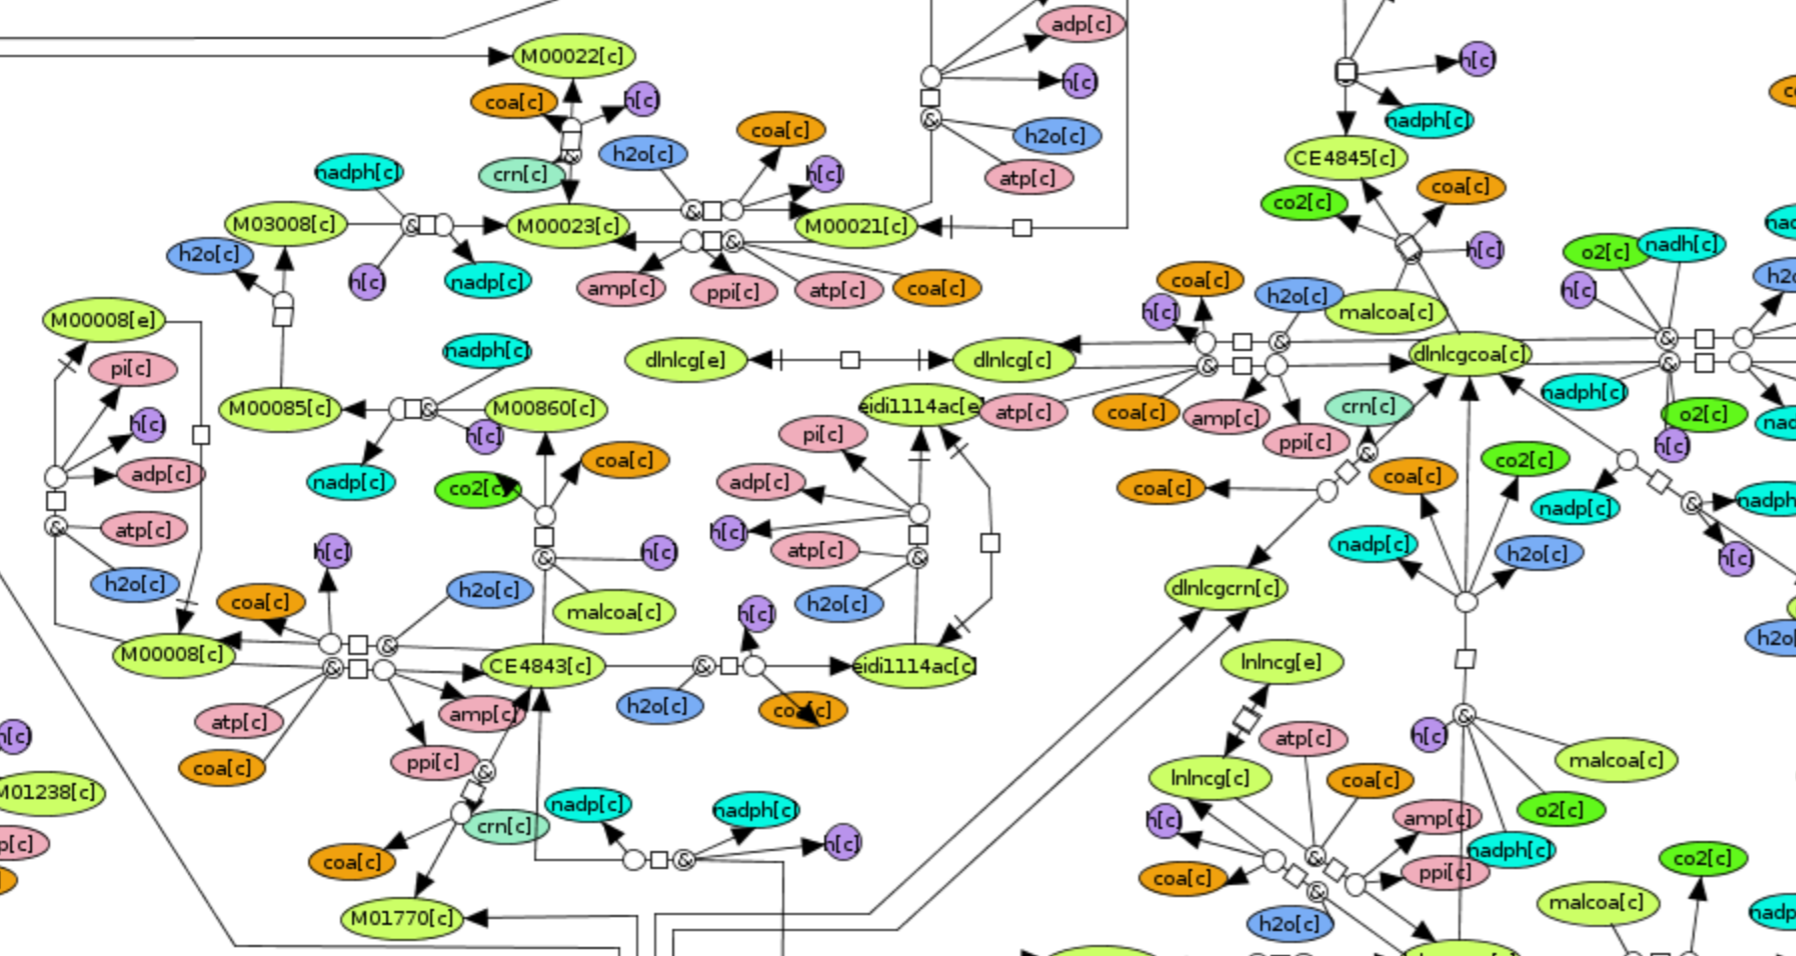
\includegraphics[width=\linewidth]{disease-map-screenshots/reconmap-zoomed.png}
      \caption{Detail view of \textit{ReconMap}}
    \end{figure}
    {\small
      \begin{itemize}
      \item some species commonly represented with unit in/out-degree
      \item \textit{ReconMap} is a vis. of a metabolic model, different char. to
        e.g. \textit{PDMap}.
      \end{itemize}
    }
  \end{frame}


  \begin{frame}

    \frametitle{Experiments / Gene Ontology Annotations / Introduction}

    \begin{columns}
      \column{10.5cm}
      \begin{itemize}
      \item True/false connectivity may not depend on graph-structural
        characteristics alone
      \item \textbf{Basic idea}: Encode biological semantics of adjacent processes
      \item e.g. $p_1$ and $p_2$ are unrelated biological processes $\leadsto$
        duplicate $S_0$?
      \end{itemize}
      \column{2.8cm}
      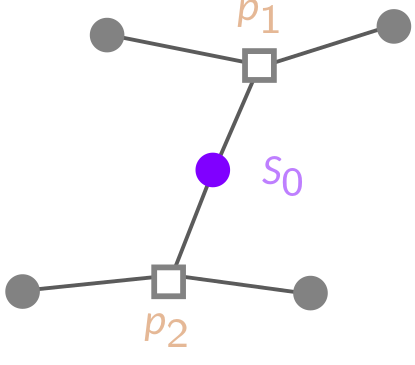
\includegraphics[width=0.7\linewidth]{true-false-connectivity-connected.png}
    \end{columns}

    \begin{columns}
      \column{0.7\linewidth}
      \begin{itemize}
      \item Species in disease maps are associated with Gene Ontology terms
      \end{itemize}
      \begin{definitionblock}{Gene Ontology}
        Directed, acyclic graph of biological \ild{terms} and their
        \ild{relationships}
        \begin{itemize}
        \item terms: molecular functions, cellular compartments, biological
          processes
        \item relationships: \cd{is-a}, \cd{part-of}, \cd{regulates}, ...
        \end{itemize}
      \end{definitionblock}
      {\small
        \begin{itemize}
        \item terms are of varying specifity, hierarchical structure
        \item here: focus on biological process subgraph
        \end{itemize}

      }
      \column{0.29\linewidth}
      \begin{figure}[h]
        \centering
        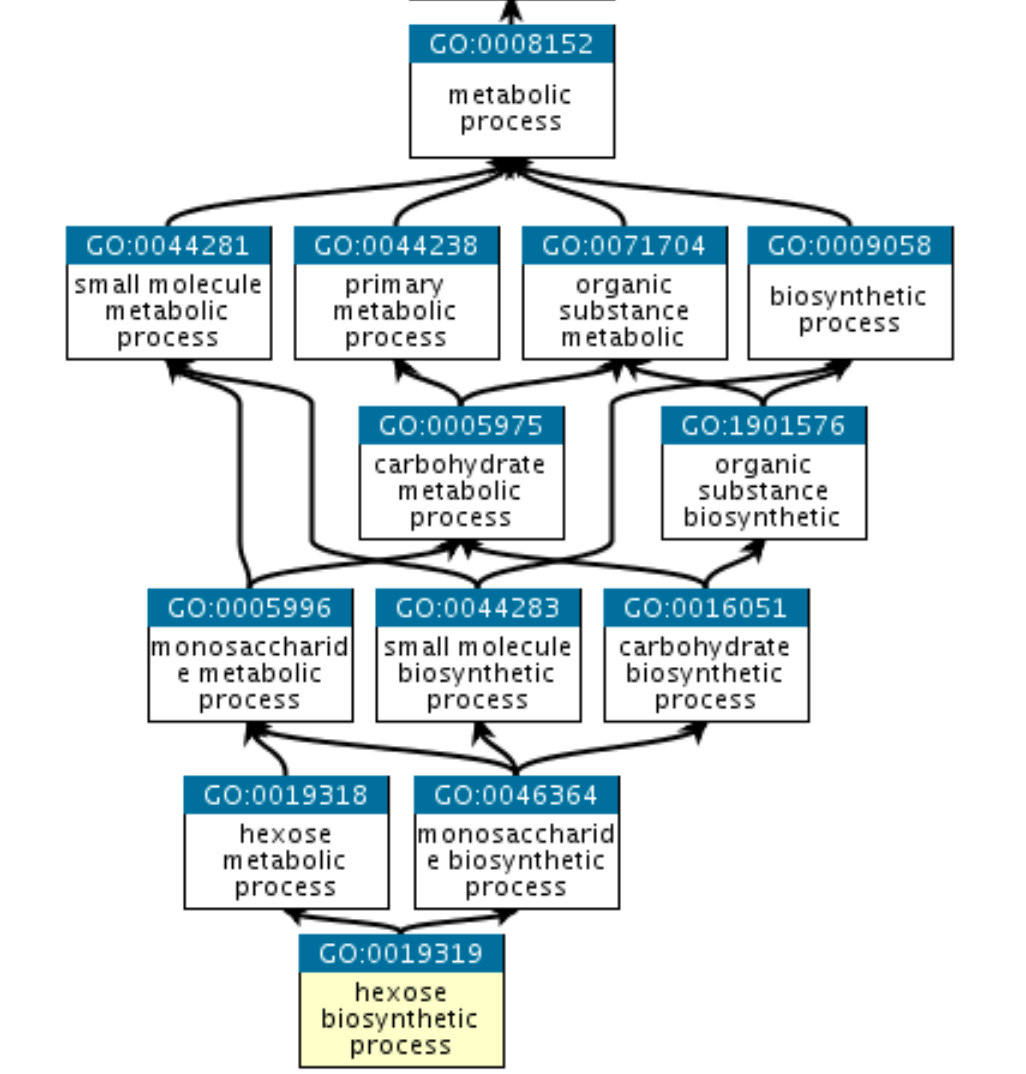
\includegraphics[width=0.95\linewidth]{GO-example.png}
        \caption{ Parent terms for a given GO term \cite{_GeneOntologyOverview_}}
      \end{figure}
    \end{columns}

    % (glycolysis involved-in carbohydrate metabolic process)


  \end{frame}

  \begin{frame}
    \frametitle{Experiments / Gene Ontology Annotations / Approach}
    % motivation for embedding-based approach
    % \begin{itemize}
    % \item How to encode GO terms?
    % \end{itemize}
    \begin{objectiveblock}{}
      Derive a fixed-length \ild{embedding} vector for each GO term s.t.
      \begin{align*}
        \text{semantic similarity of terms} \approx \text{cosine similarity of embeddings}
      \end{align*}
    \end{objectiveblock}
    {\small
      Advantages of embedding-based approach:
      \begin{itemize}
      \item Can provide embeddings directly as input feature
      \item Can handle complex species aliases by aggregating embeddings of
        contained species aliases
      \item GNNs could potentially learn complex patterns
      \end{itemize}
      % TODO compare to other approaches (see GO2vec paper)

      \begin{definitionblock}{node2vec}
        Given a simple non-attributed graph, find node embeddings s.t. for
        embeddings $\vec z_u, \vec z_v$ of nodes $u, v$
        \begin{align*}
          \vec z_u \cdot \vec z_v \approx P(\text{``$u, v$ co-occur on random walk''})
        \end{align*}
        \begin{itemize}
        \item $P(...)$ estimated by sampling random walks starting at each node
        \item Embeddings optimised via Gradient Descent
        \end{itemize}
      \end{definitionblock}
      % TODO refer to GO2Vec here
      % TODO include considerations on random walk strategy here?
      % TODO more formal definition?

    }
  \end{frame}

  \begin{frame}
    \frametitle{Experiments / Gene Ontology Annotations / Approach}

    \begin{columns}
      \column{0.6\textwidth}
      \begin{enumerate}
      \item Extract identifiers from Disease Map \\
        {\footnotesize UniProt for \textit{AlzPathway}, Entrez Gene for
          \textit{PDMap}}
      \item Obtain GO/BP graph
      \item Map identifiers to GO terms
      \item \textbf{Obtain embeddings for terms}
      \item \textbf{Map embeddings to nodes}
        \begin{itemize}
        \item Multiple terms for species: aggregate with \textit{mean}
        \item Complex species aliases: aggregate with \textit{mean}
        \end{itemize}
      \item \textbf{Create node feature}
      \end{enumerate}
      \begin{itemize}
      \item use raw embeddings
      \item measure of spread of embeddings of neighbours
      \end{itemize}
      \column{0.4\textwidth}
      \begin{figure}[h] 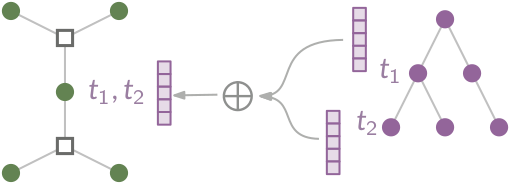
\includegraphics[width=5cm]{go-embedding.png}
      \end{figure}
    \end{columns}
    % actually finding embeddings (enumerate from written)
    % how much detail do we need to give?
    % at least mention and describe node2vec
  \end{frame}

  \begin{frame}
    \frametitle{Experiments / Gene Ontology Annotations / Results}
    % mapping from *species* to GO terms

    Use as single feature, or combined with degree.

    \begin{observationblock}{}
      \begin{itemize}
      \item No performance gain; challenges
        \begin{itemize}
        \item Quality of annotations \\
          {\footnotesize large number of annotations for some species; specifity}
        \item Quality of embeddings \\
          {\footnotesize node2vec hyperparameters}
        \end{itemize}
      \end{itemize}
    \end{observationblock}

    \begin{figure}[h]
      \centering
      \begin{subfigure}{0.40\linewidth}
        \pic{annotations/results/comparison/roc-gnn-bak.png}
        \caption{Performance of the GNN classifier on different feature sets.}
      \end{subfigure}
      \begin{subfigure}{0.40\linewidth}
        \pic{annotations/results/comparison/roc-svm-bak.png}
        \caption{Performance of the SVM classifier on different feature sets.}
      \end{subfigure}
      \caption{(\ADLast $\rightarrow$ \PDMap{}; subgraphs)}
      \label{fig:annotations-results}
    \end{figure}

    % no performance gain over baseline
    % problems with it.

    % consider/mention potential lack-of-specifity of term annotations
    % consider/mention potential 'transitivity' of term annotations?
  \end{frame}



  \begin{frame}
    \frametitle{Attachment of Edges / Introduction}
    \begin{objectiveblock}{Objective 2}
      Determine number of duplicates and attachment of edges
    \end{objectiveblock}

    \begin{itemize}
    \item[$\leadsto$] \textit{Partition} the neighbourhood of $v$.
    \item Basic idea: In a good partition, each subset of neighbours should be
      homogeneous
    \item[$\leadsto$] Find a \ild{clustering} of the neighbourhood
    \end{itemize}
    Requirements:
    \begin{itemize}
    \item Do not know number of clusters in advance
    \item Cannot assume convex clusters
    \item Assign all points to a cluster, no noise
    \item Instances can be of different scales
    \item Avoid parameters
    \item Never want single cluster or $n$ clusters
    \end{itemize}


    % requirements for classifier and why we settle for agglomerative
    % explain dendro and derivative
    % considerations on using position information

    % show real-world example and considerations on reorganisation
  \end{frame}



  \begin{frame}
    \frametitle{Attachment of Edges / Approach}

    \begin{definitionblock}{Agglomerative Clustering}
      \begin{enumerate}
      \item Initially, each point is assigned its own cluster
      \item Iteratively, two clusters with smallest inter-cluster distance $D$ are
        merged
      \item[$\leadsto$] clustering tree (\ild{dendrogram})
      \end{enumerate}
    \end{definitionblock}

    \begin{itemize}
      \small
    \item For inter-cluster distance, use \ild{single linkage}: $D(C_1, C_2) :=
      \min_{p \in C_1, q \in C_2} d(p,q)$.
    \item Treshold on max. distance inside a cluster yields concrete clustering
    \end{itemize}


  \end{frame}


  \begin{frame}
    \frametitle{Attachment of Edges / Approach}
    \begin{columns}
      \small
      \column{0.7\textwidth}
      \textbf{How to find threshold?}
      \begin{itemize}
      \item Assume clusters are density-separated
      \item[$\leadsto$] large ``step'' in distance between clusters
      \item Look for strongest increase in step size
      \end{itemize}
      \vspace{1.5em}
      \textbf{What to use as point distance measure $d$?}
      \begin{itemize}
      \item Here: position in layout \\
        {\footnotesize limited to \textit{AlzPathway reorg. steps}}
      \end{itemize}
      \column{0.3\textwidth}
      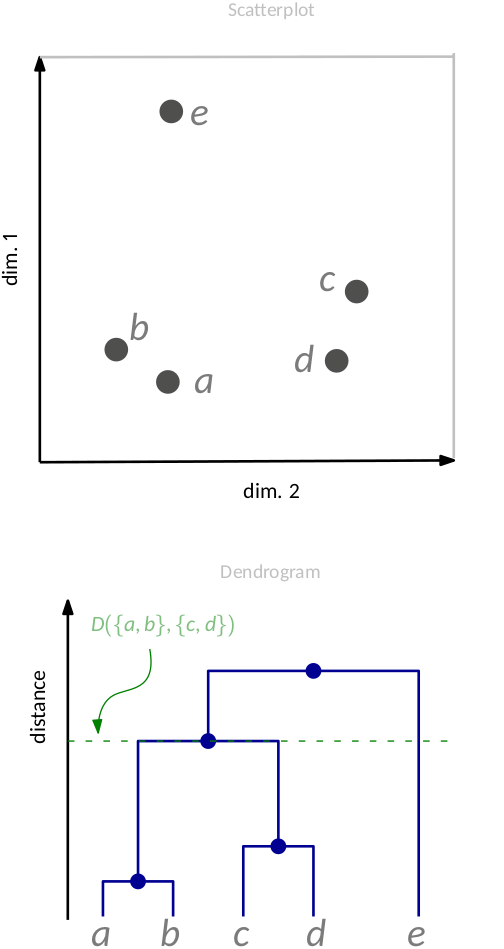
\includegraphics[width=\linewidth]{dend-motivation.png}
    \end{columns}
  \end{frame}
  % TODO why not simply consider largest step?



  \begin{frame}
    \frametitle{Attachment of Edges / Results}
    \begin{itemize}
      \small
    \item Systematic evaluation of attachment is not trivial because edges may
      have been removed in reorg. step
    \item Look at examples instead
    \end{itemize}
    \begin{observationblock}{}
      \begin{itemize}
      \item Intuitive clusterings in almost all cases
      \item May provide useful suggestions
        % TODO look at points on paper notes regarding potential examples and why
        % I did not chose them as examples
        % \item Reorganisation steps often involve more than duplications
        %   \begin{itemize}
        %   \item Re-attach to already existing duplicate
        %   \item Remove/omit a potential duplicate
        %     %     TODO more from written
        %   \end{itemize}
      \end{itemize}
    \end{observationblock}
    \begin{figure}[h]
      \centering
      \begin{subfigure}{0.48\linewidth}
        % example where it works nicely
        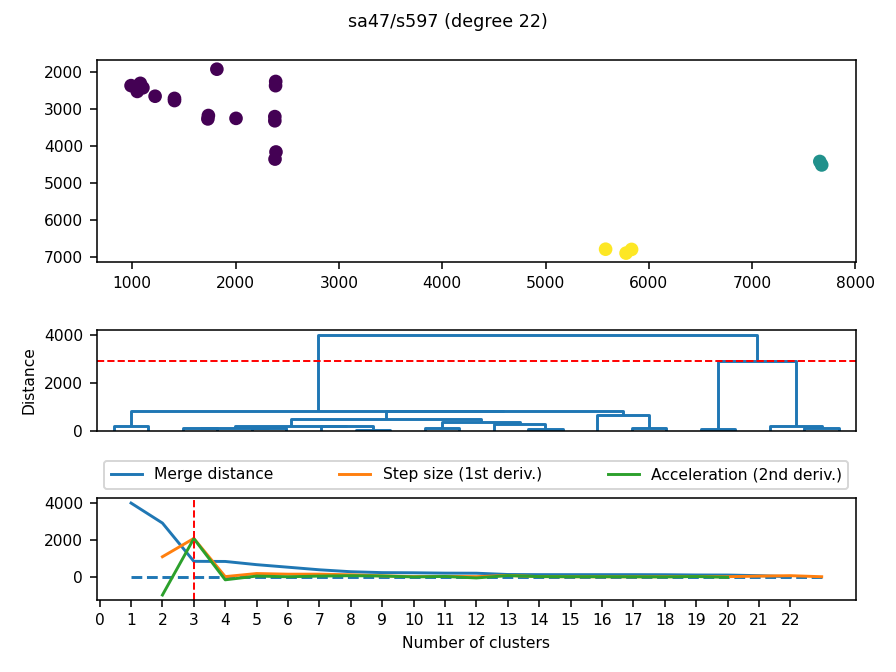
\includegraphics[width=\textwidth]{attachment-examples/s597/dendrogram.png}
        % \caption{
        % Simple example for which our method yields an intuitive clustering. This
        % case is shown on the actual disease map in \reffig{reorg-duplication-example}.
        % }
        \label{fig:s597-dendrogram}
      \end{subfigure}
      %
      \begin{subfigure}{0.48\linewidth}
        \includegraphics[width=\textwidth]{AlzPathwayReorg202-203/sa89.png}
        % \caption{Example in which using the second derivative yields a clustering
        % that intuitively seems more reasonable. The first derivative has its
        % maximum at 3 clusters.
        % }
        \label{fig:dendro-b}
      \end{subfigure}
      % \caption{
      % Examples for the clustering procedure described in \refsec{edge-attachment}.
      % The topmost scatterplot shows the positions of neighbours
      % of a target node in the layout (target node and edges are not shown; note that
      % $x$ and $y$-axes have different scales). Below, a clustering dendrogram describes
      % the distances between any two clusters as they were merged. Finally, the
      % sequence of merge distances as well as its first and second derivative are shown.
      % Taking the maximum yields a hint for the number of clusters
      % to choose. The red line indicates the suggested choice for the number of
      % clusters and thus a concrete clustering.
      %   % , determing the merge node in the
      %   % dendrogram where the ``cut'' should be made.
      % All examples are from \textit{AlzPathway} reorganisation steps and
      % and correspond to aliases that were actually duplicated}
      % \label{fig:neighb-clust-examples}
    \end{figure}
  \end{frame}

  \begin{frame}
    Compare suggestion to real reorganisation step
    \begin{itemize}
    \item Many other reorganisations in neighbourhood (nodes, edges added and removed)
    \item Neighbours reattached to other already existing alias of same species
    \item Here: more duplicates than indicated by clustering were introduced
    \end{itemize}
  \end{frame}



  \begin{frame}
    \begin{figure}[h]
      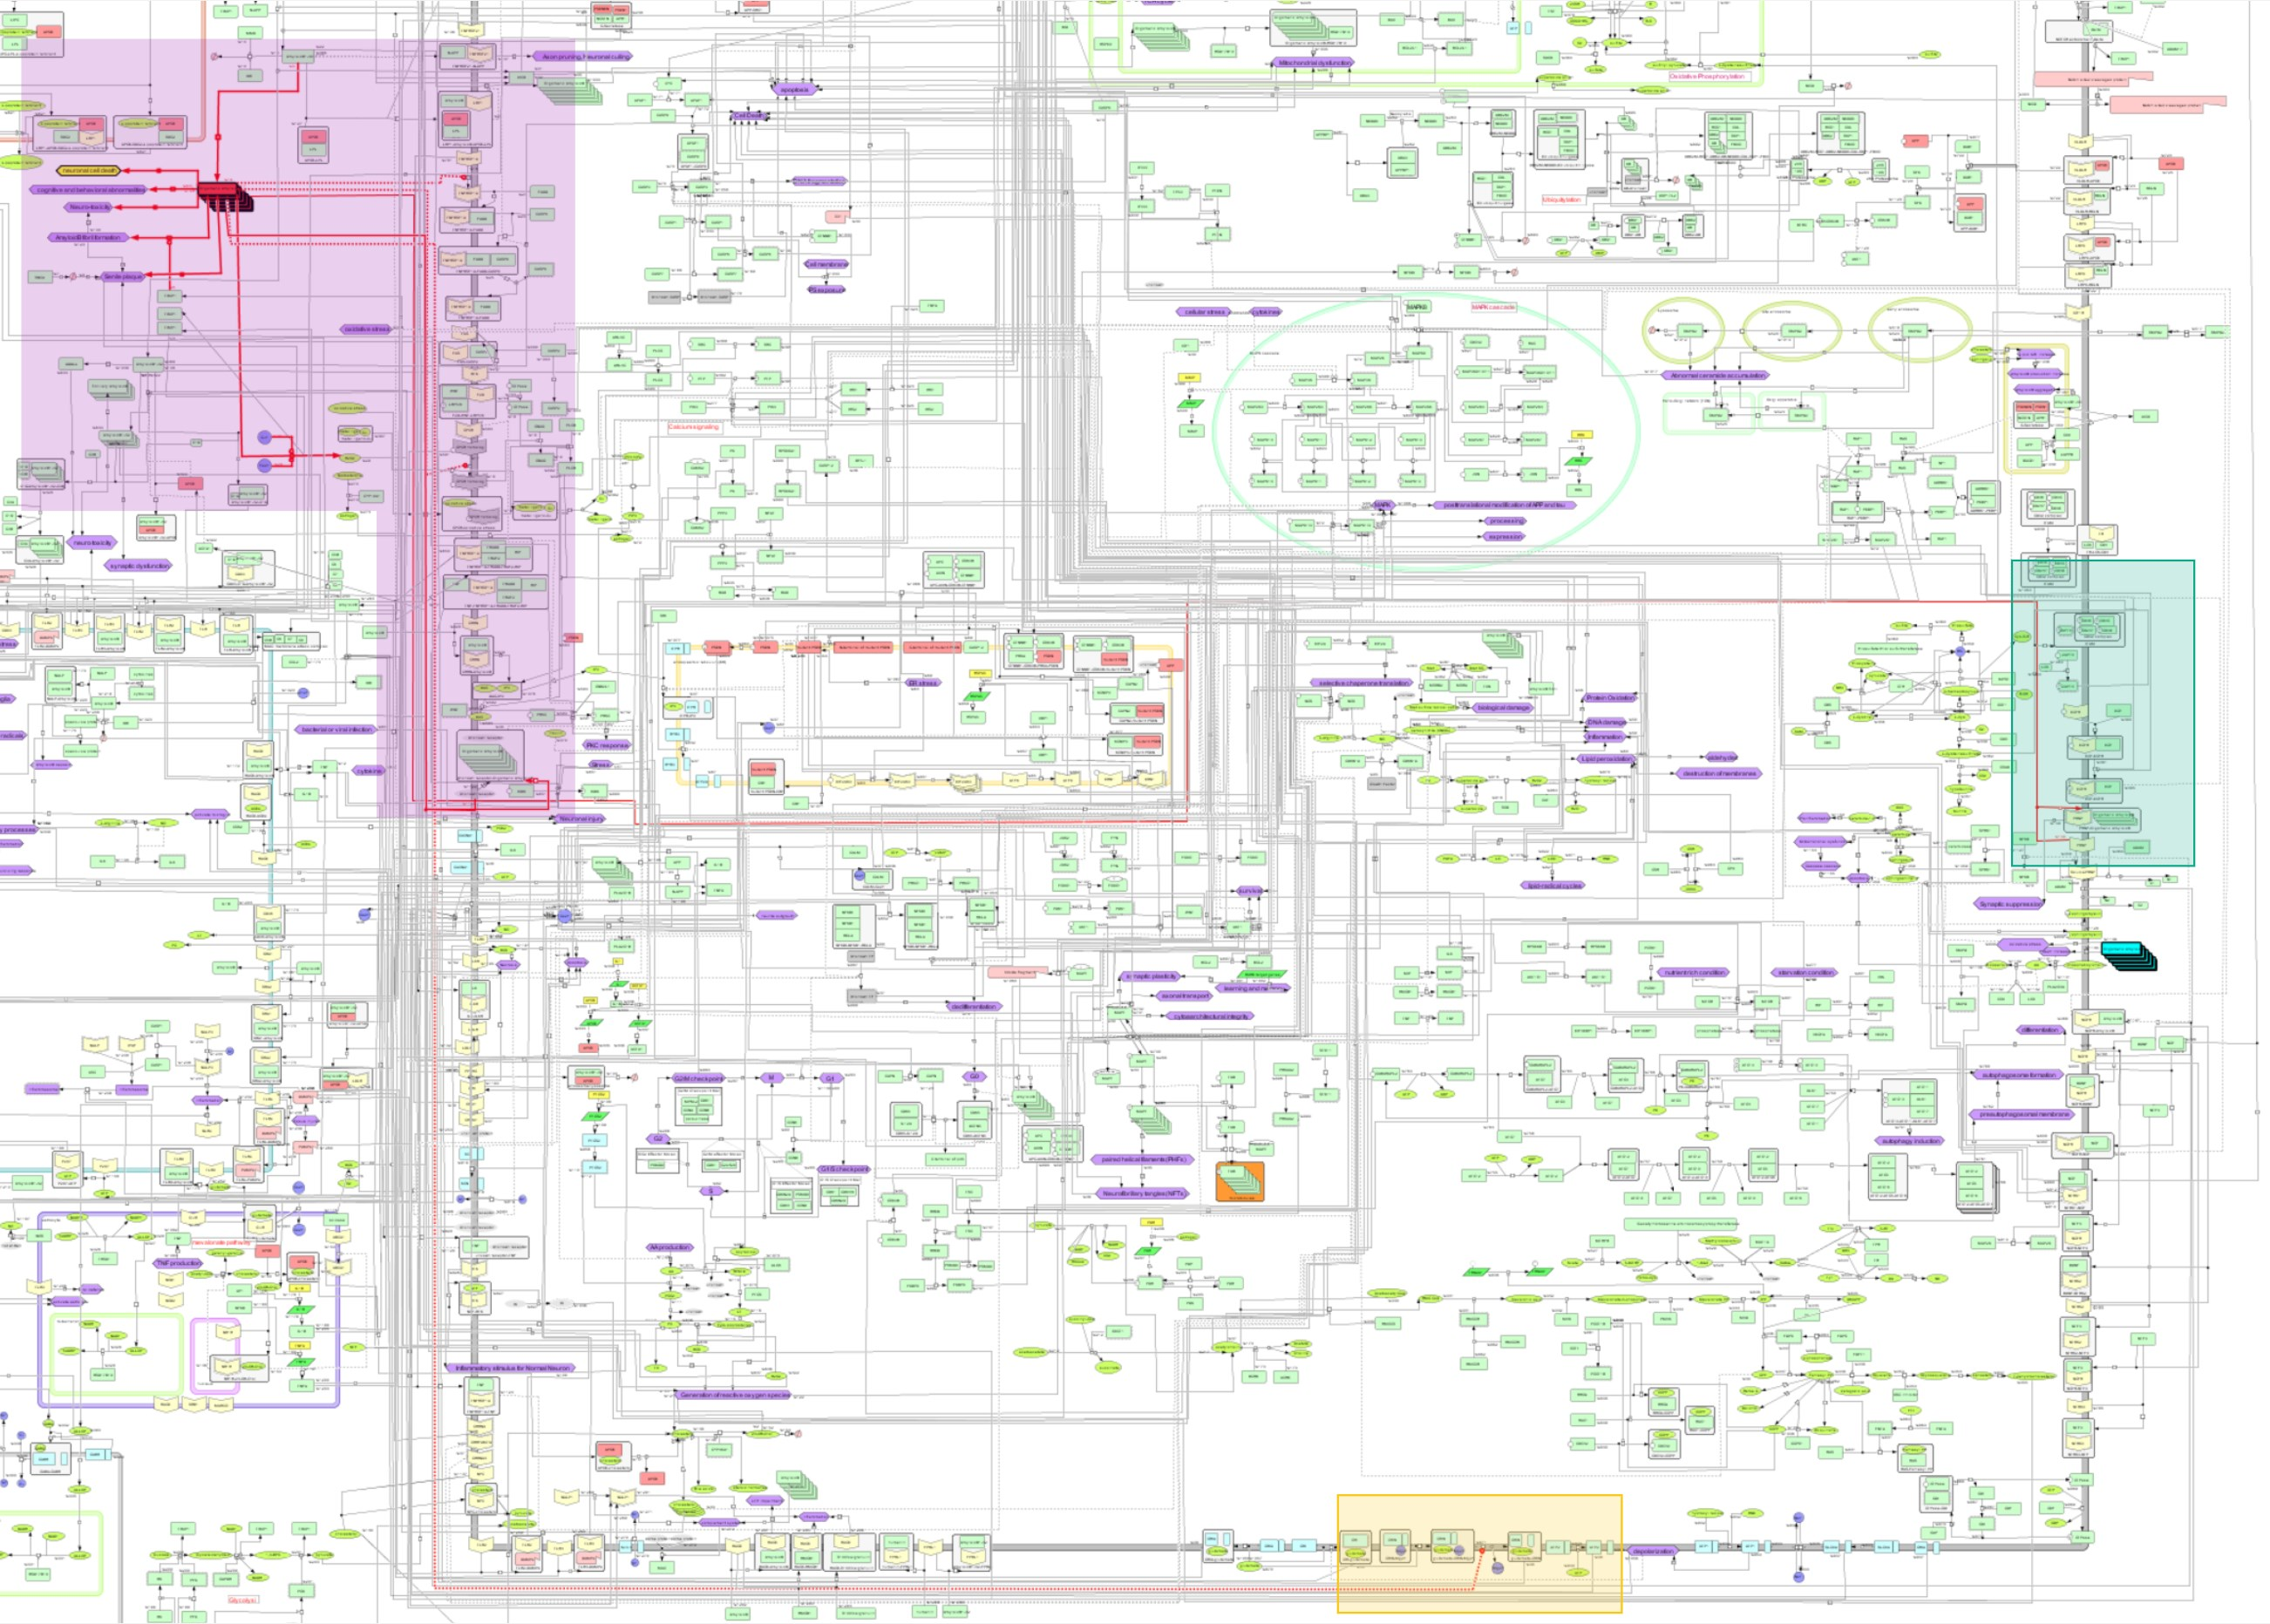
\includegraphics[height=\textheight]{attachment-examples/s597/202.jpg}
      \pause
      % \caption{Example of a real reorganisation step that duplicates a species
      % alias. The graphic is described in detail in \refsec{attachment-of-edges}.
      % }
      %   \label{fig:reorg-duplication-example}
    \end{figure}

  \end{frame}


  \begin{frame}
    \begin{figure}[h]
      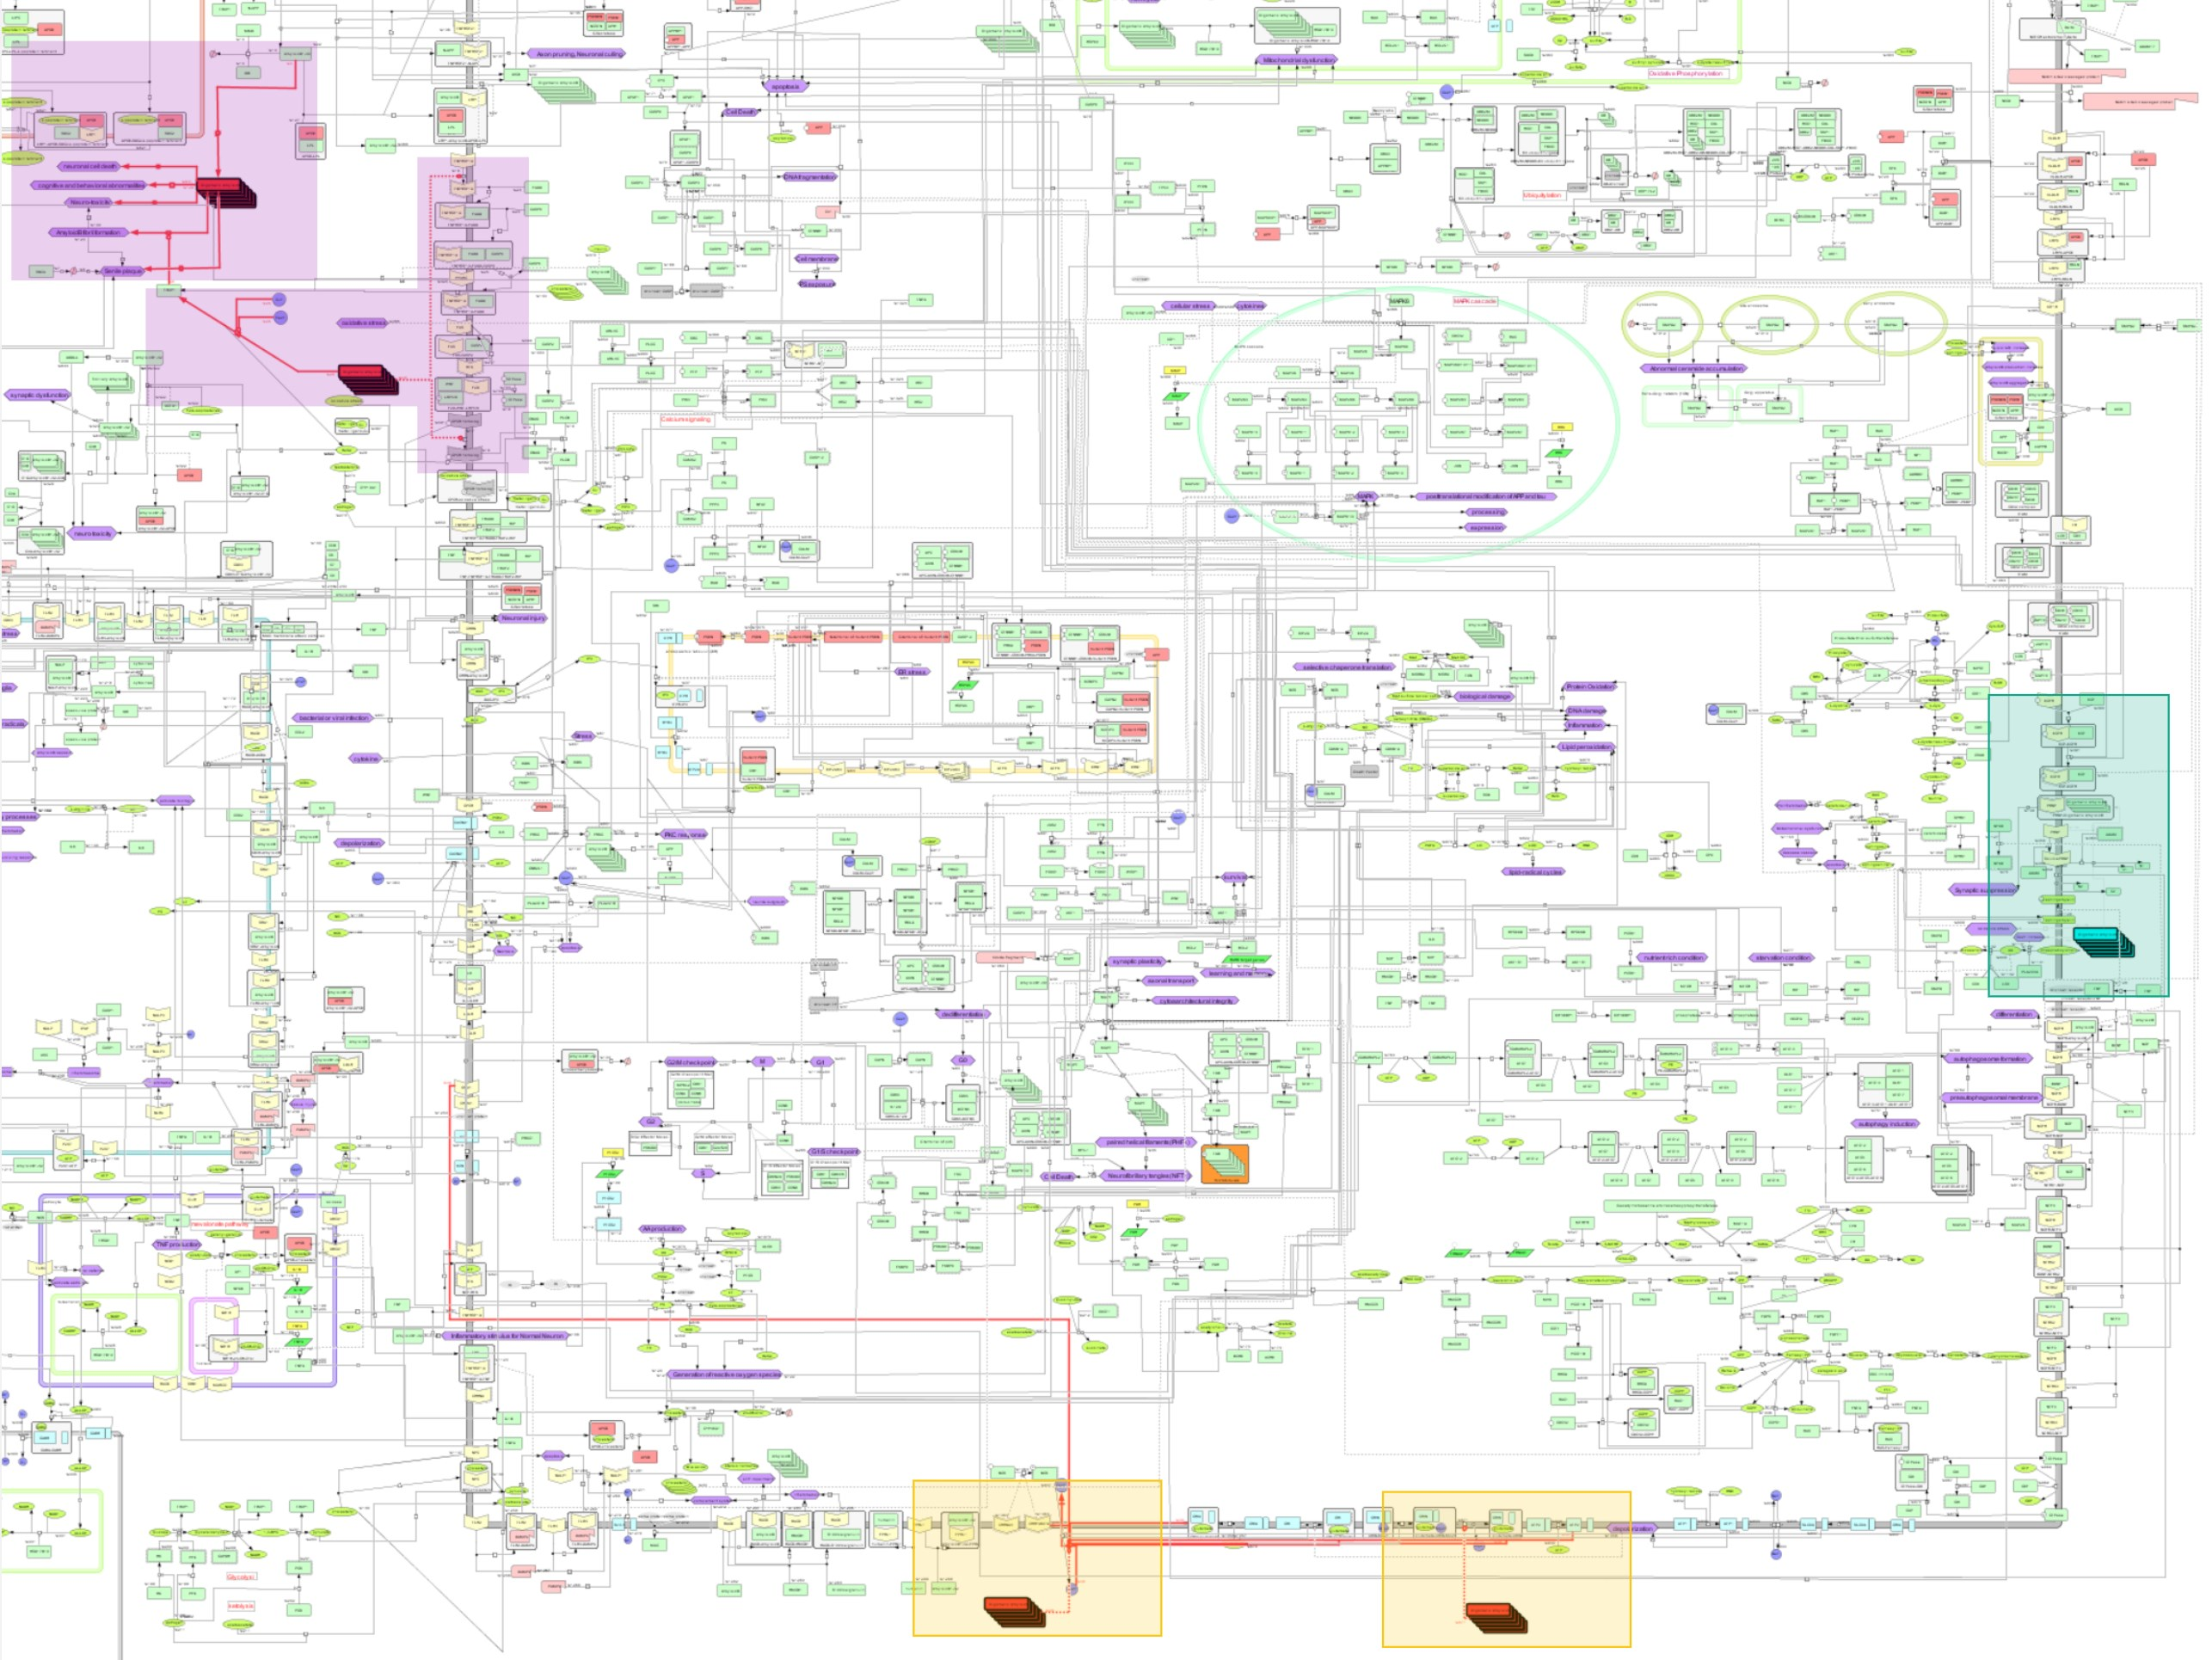
\includegraphics[height=\textheight]{attachment-examples/s597/203.jpg}
      % \caption{Example of a real reorganisation step that duplicates a species
      % alias. The graphic is described in detail in \refsec{attachment-of-edges}.
      % }
      %   \label{fig:reorg-duplication-example}
    \end{figure}

  \end{frame}








  \begin{frame}
    \frametitle{Conclusion / Results \& Discussion 1}

    \pause

    \begin{resultblock}{}
      \textbf{    Simplify machine learning task while maintaining same performance}
      \begin{itemize}
      \item \textbf{reorganisation steps not essential} \\
        {\footnotesize hard to obtain in practice}
      \item need not compute structural features on both simple and bipartite
        graph \\
        {\footnotesize substantial computational cost for large networks}
      \end{itemize}
    \end{resultblock}

    \pause

    \begin{resultblock}{}
      \textbf{Using directed degree as feature yields good performance}
      \begin{itemize}
      \item ... but other structural features yet improve classifier performance
        slightly
      \item Supports previous work from a different angle: Degrees also useful to
        model given decisions of expert
      \end{itemize}
    \end{resultblock}

    \pause

    \begin{resultblock}{}
      \textbf{NNs slightly outperform SVM classifiers}
      \begin{itemize}
      \item Open how useful this advantage is in practice
      \item No gain through message-passing (in this implementation)
      \end{itemize}
    \end{resultblock}

  \end{frame}

  \begin{frame}

    \begin{resultblock}{}
      \frametitle{Conclusion / Results \& Discussion 2}
      Embedding-based approach to encode \textbf{Gene Ontology term annotations as node
        features}
      \begin{itemize}
      \item Not useful in this implementation
      \item ... % TODO challenges with this
      \end{itemize}
    \end{resultblock}


    \pause

    \begin{resultblock}{}
      Suggestions on number of duplicates and edge attachment: \textbf{agglomerative
        clustering approach provides reasonable results}
    \end{resultblock}

  \end{frame}


  % TODO few general sentences on problem of node duplication and ML
  % - reorganisation often involves not only duplication?

  \begin{frame}
    \frametitle{Challenges}
    % - reorganisation steps contain much more than only duplications

    % TODO also technical challenges here? maybe as bonus slide
  \end{frame}


  \begin{frame}
    \frametitle{Future Work}
    % reconsider use-case -- maybe then train & evaluate on reorganisation steps

    % more training data

    % features
    % layout-based features
    % semantic:
    % - more work on GO annots
    % - compartment membership
    % - CD roles in reactions (promising)
    % - compare to simpler classifier or simply degree threshold

  \end{frame}



  \begin{frame}
    \centering
    Thanks for listening\\[1.15em]
    \Laughey[1.4] \\
    % 
\includegraphics[width=1.5em]{laughey.png}
  \end{frame}



  \begin{frame}
    \frametitle{Additional examples for Clustering}

    \begin{figure}[h]
      \centering
      \begin{subfigure}{0.48\linewidth}
        % example where distributions are tricky (obs) sa25 sa102 sa123
        \includegraphics[width=\textwidth]{AlzPathwayReorg202-203/sa102.png}
        % \caption{Distances between the yellow points are not much different from
        % the distance between the purple and the yellow clusters (as measured by
        % single linkage). While the heuristic yields only two clusters, it may
        % have also been feasible to create many clusters. }
        % \label{fig:dendro-c}
        % or sa77
      \end{subfigure}
      \begin{subfigure}{0.48\linewidth}
        \includegraphics[width=\textwidth]{AlzPathwayReorg202-203/sa74.png}
        % \caption{ Example illustrating the ability of single linkage clustering to
        % identify non-convex clusters. In this case, introducing a single
        % duplicate for large green cluster is probably not sufficient. }
        % \label{fig:dendro-d}
      \end{subfigure}
    \end{figure}
  \end{frame}


  \section{References}

  \begin{frame}[allowframebreaks]
    % \nocite{*}
    \footnotesize
    % \bibliographystyle{unsrt} % sort by appereance in text
    % \bibliography{../written/BA.bib}
    \printbibliography
  \end{frame}

\end{document}
